\documentclass[a4paper,french,12pt]{report}
\usepackage[utf8]{inputenc} % Encodage du fichier
\usepackage[T1]{fontenc} % Encodage des fonts nécessaire pour le Latin
\usepackage[english,frenchb]{babel} % Pour changer la langue des mots générés et choisir la bonne mise en page
\usepackage{lmodern} % Le latin modèrne
\usepackage[top=2cm, bottom=2cm, left=3cm, right=2cm]{geometry} % Définir les marges de la page
\usepackage[hidelinks,
            urlcolor=blue,
            unicode=true,
            pdftitle={},
            pdfauthor={Hamza ABBAD}
            pdfdisplaydoctitle=true]{hyperref} % Pour les liens
\usepackage{fancyhdr} % Pour le style de la page
\usepackage[font=it]{caption} % Rendre les titres des tableaux italiques
\usepackage{microtype}
\usepackage{graphicx} % Pour les images
\usepackage{subcaption} % Pour mettre plusieurs images sur la même ligne
\usepackage{float} % Pour empêcher le déplacement des tableaux et des figures.
\usepackage{babelbib} % Pour changer la langue dans la bibliographie

\graphicspath{ {pictures/} } % Spécifier le répertoire contenant les images
\DisableLigatures[f]{encoding=*}
\renewcommand \thechapter{\Roman{chapter}} % Utiliser les numéros romans pour les chapitres
\captionsetup{labelfont=it,textfont=it,labelsep=period}
\AtBeginDocument{ % Changer les légendes
  \renewcommand\tablename{\itshape Tableau}
  \renewcommand{\figurename}{\itshape Figure}
	% Renommer la table des matières
	\renewcommand{\contentsname}{Sommaire}
}


\date{}
% Style de l'entête et le pied de la page
\setlength{\headheight}{16pt}
\pagestyle{fancyplain}
\lhead{} % Enlever la section
\rhead{\fancyplain{}{\footnotesize \itshape{\nouppercase{\leftmark}}}} % Titre du chapitre en miniscule avec taille 10
\cfoot{} % Déplacer le numéro de la page
\rfoot{\fancyplain{\thepage}{\thepage}} % à droite de la page

% Espace entre les lignes
\linespread{1.3}

\begin{document}
% Indexes
% \tableofcontents
% \listoffigures

\setlength{\parskip}{0.6em plus 0.1em minus 0.1em}

% Changer le style des listes de descriptions
\let\olddescription\description
\let\endolddescription\enddescription
\renewenvironment{description}{
\let\olditem\item
\renewcommand\item[2][]{\olditem[\textit{##1}] ##2}
\begin{olddescription}}
{\end{olddescription}\ignorespacesafterend}

% Redéfinition des chapitres et sections pour les inclure dans le sommaire
\makeatletter
\let\oldchapter\chapter
\newcommand{\@chapterstar}[1]{\cleardoublepage\phantomsection\addcontentsline{toc}{chapter}{#1}{\oldchapter*{#1}}}
\newcommand{\@chapternostar}[1]{{\oldchapter{#1}}}
\renewcommand{\chapter}{\@ifstar{\@chapterstar}{\@chapternostar}}
\let\oldsection\section
\newcommand{\@sectionstar}[1]{\phantomsection\addcontentsline{toc}{section}{#1}{\oldsection*{#1}}}
\newcommand{\@sectionnostar}[1]{{\oldsection{#1}}}
\renewcommand\section{\@ifstar{\@sectionstar}{\@sectionnostar}}
\makeatother

% Changer les captions pour cacher les références dans la table des figures
\let\oldcaption\caption
\renewcommand{\caption}[2]{\oldcaption[#1]{#1#2}}

% Mes commandes
\newcommand{\keyword}[1]{\emph{#1}}

% \chapter*{Introduction générale}

L'être humain, en utilisant ses yeux et son cerveau, est capable de distinguer facilement
entre les niveaux de distances de différents objets qui se trouvent dans une scène.
Par contre, les machines programmables, comme les ordinateurs, ne disposent d'aucune
méthode algorithmique qui leur permette de ce faire à partir des images bidimensionnelles
reçues à travers les caméras ordinaires.

L'extraction des profondeurs d'une image 2D, ou l'estimation de la distance
d'un objet par rapport à la caméra, font partie des problèmes appartenant à une catégorie
connue dans le domaine de la vision par ordinateur. Plusieurs approches ont été
proposées pour les résoudre, chacune ayant ses propres contraintes, avantages, et
inconvénients.

La méthode utilisée dans ce travail est basée sur \keyword{l'apprentissage automatique
supervisé} dont le principe est d'utiliser un ensemble de données contenant les
images et les profondeurs correspondantes. Son avantage majeur est de pouvoir
produire un modèle permettant d'estimer les profondeurs sans avoir à implémenter
les détails du traitement explicitement.

Cependant, ces méthodes nécessitent
un nombre considérable de données afin de pouvoir fonctionner correctement.
L'obtention des données et la correspondance entre les entrées et les sorties
est un travail qui se fait généralement de façon manuelle dans la majorité des tâches
et qui demande un effort important du côté des constructeurs de l'ensemble. C'est la
raison pour laquelle la majorité des travaux qui concernent l'apprentissage automatique
utilisent des ensembles prêts, préparés dans des travaux antérieurs (par exemple
MNIST~\cite{lecun2010mnist} et CIFAR-10~\cite{krizhevsky2009learning}).

En effet, dans certaines tâches, la génération de cet ensemble peut être automatisée
et donc toutes les opérations précédentes sont effectuées par des programmes au lieu
des personnes. Cela fait partie des méthodes de \keyword{l'apprentissage
automatique auto-supervisé} qui n'est qu'un cas spécial de celui supervisé où
l'ensemble de données est construit automatiquement.

C'est dans ce contexte que se situe notre travail, qui combine deux
grandes tâches : d'abord, générer un ensemble de données contenant les images et les distances
des obstacles correspondantes après avoir construit une machine mobile permettant
de ce faire; ensuite, concevoir un modèle d'apprentissage automatique et utiliser
l'ensemble de données pour effectuer son entraînement.

Contrairement aux travaux
antérieurs, la première tâche est réalisée ici en utilisant des capteurs ultrasoniques
et non pas des capteurs lasers. Les modèles conçus dans la deuxième tâche sont
des réseaux de neurones convolutionnels.

Nous avons organisé le mémoire comme suit.
D'abord, un chapitre contenant des concepts de base et des notions générales dans
les domaines de la robotique, la vision par ordinateur, et l'apprentissage automatique.
Ensuite, un deuxième chapitre consacré à l'exposition de quelques travaux précédents
autour de notre sujet. Le troisième présente les parties
matérielles et logicielles de notre machine et explique son fonctionnement.
Le quatrième décrit les structures de nos données et les
architectures de nos réseaux convolutionnels. Le dernier présente
les exécutions d'apprentissage que nous avons lancées et les résultats recueillis
de nos tests.

\chapter{Concepts de base}

\section*{Introduction}

Ce chapitre représente une brièvement la robotique, et
l'apprentissage automatique. Il contient quelques définitions et explications
concernant les notions principales de robotique et d'apprentissage automatique
qui sont requises pour ce sujet.

\section{Robotique}

La \textbf{robotique}\footnote{\url{https://en.wikipedia.com/wiki/Robotics}}
est une discipline qui fait partie de la mécanique, de
l'électrique, et l'informatique en même temps. Elle s'intéresse à la conception,
à la construction et au fonctionnement des \emph{robots}, ainsi que la création
des systèmes informatiques qui les contrôlent.

\subsection{Le robot}

Le mot \textbf{robot} refère à un agent électromécanique autonome ou
semi-autonome, guidé par un programme informatique ou un circuit électronique.

Ce terme a été publiquement utilisé pour la première fois par l'écrivain tchèque
Karel Čapek en 1920 dans sa pièce de théâtre \emph{R.U.R.
(Rossum's Universal Robots)}.

Il existe plusieurs types de robots répondant à différents fonctions. Nous
citons les plus importants.

\begin{itemize}
  \item Les robots mobiles ont la possibilité de se déplacer dans leur
  environnement pour accomplir leurs tâches.
  \item Les robots industriels sont construits à partir de bras jointés et
  sont utilisés dans les lignes de production.
  \item Les robots de service ont un rôle proche de celui des robots
  industriels, sauf qu'ils sont utilisés pour fournir des services autres que
  la production.
  \item Les robots éducationnels sont utilisés comme des assistants
  éducationnels pour les enseignants afin d'aider les élèves à mieux comprendre
  des concepts mathématiques, physiques, électroniques et programmatifs.
\end{itemize}

La structure d'un robot comporte trois éléments de point de vue construction.

\begin{itemize}
  \item \emph{Sur le plan mécanique}, tous les robots sont conçus pour leurs
  permettre d'accomplir leurs
  tâches. Cette construction dépend du type de la machine et de l'environnement
  où elle fonctionne. Elle définit la forme extérieure et la structure interne
  du robot.
  \item \emph{Sur le plan électrique}, un robot a besoin de composants
  électriques qui lui offrent la possibilité de
  contrôler son corps mécanique et de capturer les caractéristiques de son
  environnement.
  \item \emph{Sur le plan programmatif}, chaque robot doit avoir un certain
  niveau de programmation qui le permet de
  savoir comment réaliser une opération ou prendre une décision. Cette
  programmation peut être réalisée par une combinaison des circuits intégrés dans
  les cas simples, ou à l'aide d'une série d'instructions exécutées sur un
  microprocesseur dans les cas les plus complexes.
\end{itemize}

\subsection{Les modules électroniques}
Un module est un circuit spécialisé pour réaliser une tâche donnée. Chaque
module contient tous les composants électroniques nécessaires pour son
fonctionnement et sa connexion avec les autres modules.

\begin{description}
  \item[\emph{Le microcontrôleur}] est un module électronique programmable ayant une capacité
  limitée de traitement de données. Il inclut un microprocesseur, une mémoire
  centrale et une mémoire secondaire à lecture seule mais reinitialisable.
  Il peut lire les données reçues des autres modules et leurs envoyer des commandes
  pour contrôler leurs fonctionnement à travers ses ports. Chaque système embarqué
  contient au moins un microcontrôleur.
  \item[\emph{Les capteurs}] sont des modules qui permettent d'obtenir des données sur
  l'environnement sous forme d'un signal électrique numérique ou analogique.
  Parmi ces capteurs, on trouve les capteurs de la température qui mesure le degré
  de la température de l'environnement où il se trouve. Il y a aussi les capteurs
  ultrasoniques permettant d'envoyer et de recevoir un ultrason. Il sont utilisés
  fréquemment pour le calcul de la distance en mesurant le temps écoulé entre
  l'envoi et la réception du signal.
  \item[\emph{Les moteurs}] sont les composants qui transforment l'énergie électrique en
  mouvement mécanique. Ils tournent dans un seul sens et à une vitesse qui
  sont déterminés respectivement par le sens et l'intensité du courant électrique.
\end{description}

\section{Apprentissage automatique}

L'apprentissage automatique (\emph{machine learning}) est une filière de
l'intelligence artificielle qui s'intérresse aux techniques de conception des
modèles ayant la capacité d'apprendre à réaliser une tâche sans les programmer
explicitement. Il y existe de nombreuses méthodes, chacune appartenant à
une des trois classes :
\emph{l'apprentissage supervisé}, \emph{l'apprentissage non supervisé}, et
\emph{l'apprentissage par renforcement}.
Pour le présent travail, c'est l'apprentissage supervisé qui est nécessaire.

\subsection{Apprentissage supervisé}

C'est un mode permettant de trouver une approximation d'une fonction en utilisant
les données avec les résultats attendus de cette fonction. Un modèle approximant
la fonction sera généré en utilisant une des techniques de ce mode. Une fois que
le modèle est entraîné, il serait capable d'opérer sur de nouvelles données qui
n'ont pas été vues lors de l'apprentissage. Parmi ces techniques on trouve
\emph{les réseaux de neuronnes artificiels} auxquelles nous avons recours dans
ce projet.

C'est une technique inspirée du cerveau humain. Son architecture est composée de
plusieurs \emph{couches} dont chacune contient plusieurs unités de calcul dites
\emph{perceptrons}.
Il existe des connexions entre les perceptrons. Le nombre et le type de ces
connexions dépend du type du réseau et il y a plusieurs types de réseaux de
neuronnes possibles, chaque type étant adapté a un type de problèmes.

Dans les
problèmes liés aux images, le type préféré est celui des \emph{réseaux convolutionels}
dont nous nous servirons et que nous détaillons au point suivant.

\section{Les réseaux convolutionels}

Ce type de réseaux se compose de trois couches de
types différents : les \emph{couches convolutionelles}, les
\emph{couches de regroupement (mise en commun)} et les
\emph{couches entièrement connectées (denses)}.

\subsection{Couches convolutionelles}

Chaque perceptron dans une couche de convolution est relié seulement à un petit
sous ensemble de perceptrons de la couche précédente. Cet ensemble représente
une région rectangulaire dans une image. L'image peut être l'originale ou
bien la résultante des opérations des couches précédentes. La fonction générant
chaque région est appelée le \emph{filtre}. Ce type de couches est généralement
placé au début et au milieu du réseau.

Chaque couche convolutionelle nécessite des hyperparamètres qui doivent
être fixés dans la conception : la taille spatiale du filtre $F$ et la
profondeur du filtre $K$, le pas de la convolution $S$, le rembourrage par zero
$P$, et fonction d'activation.

\begin{description}
  \item[\emph{La taille spatiale du filtre $F$}] sert à
  spécifier le nombre d'entrées pour chaque perceptron,
  \emph{\textbf{la profondeur du filtre $K$}} spécifie
  le nombre de matrices de poids partagés.
  \item[\emph{Le pas de la convolution $S$}] est la différence entre le bord d'un
  filtre et le même bord du filtre du perceptron successif.
  \item[\emph{Le rembourrage par zero $P$}] permet d'entourer
  l'entrée par des pixels nuls avant d'appliquer la convolution pour maintenir
  sa taille.
  \item[\emph{La fonction d'activation}] qui, à la sortie de chaque couche, permet grâce
  à une fonction mathématique de modifier les valeurs avant de les transmettre à la
  couche suivante.
\end{description}

\subsection{Couches de regroupement}

Le rôle de ces couches est de réduire la taille spatiale du résultat des couches
précédentes en gardant l'information essentielle. Cette opération est souvant
appliquée en utilisant la valeur maximale entre les pixels ou par le calcul de
la moyenne. Ces couches sont généralement placés après les couches
convolutionelles.

Les hyperparamètres requis pour cette couche sont les mêmes que ceux des couches
convolutionelles auxquelles il faut ajouter la La fonction du regroupement
(maximum ou moyenne).

\subsection{Couches entièrement connectées}

C'est le type classique des couches dans un réseau de neuronnes artificiels.
Chaque perceptron dans ce type est connecté à tous les perceptrons de la couche
précédente. Ces couches sont utilisées à la fin du réseau.

Les hyperparamètres nécessaires pour ce type :

\begin{itemize}
  \item le nombre de perceptrons $K$,
  \item la fonction d'activation.
\end{itemize}

\section*{Conclusion}

Ce chapitre a été consacré aux notions de la robotique et l'intelligence
artificielle requises pour la compréhension du sujet. Le chapitre suivant fera
la description matérielle et logicielle de la réalisation présentée.

% Changer les captions pour cacher les références dans la table des figures
\let\caption\oldcaption
\chapter{\'Etat de l'art}

\setcounter{chapter}{1} % Forcer la numérotation pour les compilations à un seul chapitre

\section{Introduction}

L'estimation de la distance à partir des images d'une scène est un problème
fondamental dans la vision artificielle et qui a été étudié depuis longtemps.
Beaucoup d'approches ont été proposées.

Ces approches se répartissent en deux catégories : les méthodes qui sont basées
sur la vision binoculaire et les méthodes basées sur la vision monoculaire.
Les méthodes binoculaires utilisent deux cameras et calculent la distance
en connaissant la position et l'orientation de chaque camera dans la scène
par l'utilisation de principes géométriques comme la triangulation. Les
méthodes basées sur la vision monoculaire qui estiment la distance d'une seule
image par l'extraction de certains caractéristiques de l'image comme la
distribution de la brume et les points de fuite, ou par l'utilisation des
techniques d'apprentissage automatique.

Pour des raisons historiques, la plupart des recherches portant sur l'estimation
de distances ont été basées sur la vision binoculaire ou sur l'utilisation de
plusieurs images, ou encore sur l'utilisation des caractéristiques bien définies
dans la vision monoculaire. Cependant, les dernières années ont connu
l'émergence d'approches basées sur l'apprentissage automatique.
Dans ce chapitre nous présentons ce que nous avons trouvé comme travaux basés
sur l'utilisation des techniques d'apprentissage automatique.

\section{\'Evitement d'obstacles par la vision monoculaire}

L'un des premiers travaux utilisant l'apprentissage automatique et qui ont eu
des résultats satisfaisants est celui de Michels et al.\cite{michels2005high}
qui ont développé une méthode pour permettre à une voiture télécommandée de
naviguer de façon autonome dans un environnement non structuré à une haute
vitesse ($5m/s$).

Dans leur approche ils ont utilisé deux types d'apprentissage : l'apprentissage
supervisé pour estimer les distances des obstacles figurant dans l'image de la
camera, et l'apprentissage par renforcement afin de calculer le degré de
changement de la direction du mouvement. Ce dernier utilise les distances résultantes
du premier apprentissage pour choisir la direction.

Dans la première étape, ils ont construit une plateforme constituée d'un
scanner laser de distances, d'une webcam et d'un ordinateur portable qui commande
ces périphiriques et traite les données qui les génèrent. Cette plateforme se
déplace continuellement dans une forêt pour prendre les photos de
l'environnement et les mesures de distance respectives.

\begin{figure}[H]
\begin{center}
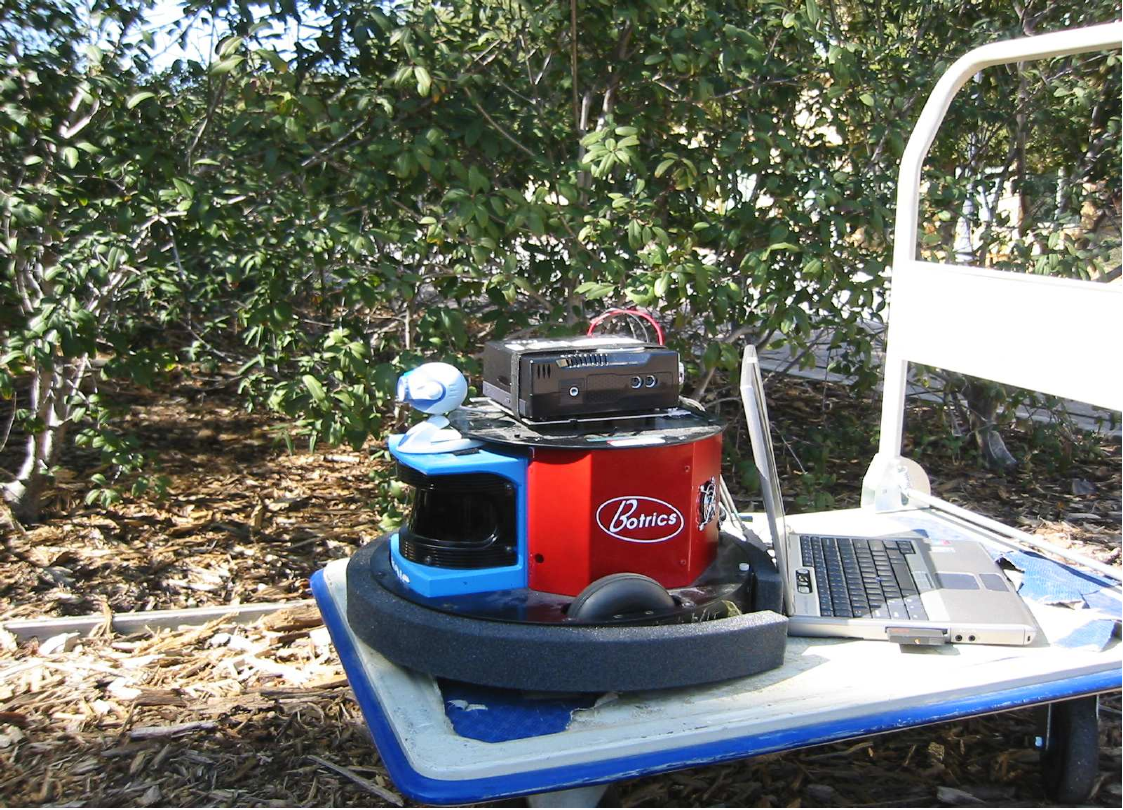
\includegraphics[width=0.7\textwidth]{HighSpeedObstacleAvoidanceRig}
\caption{La plateforme qui prend les mesures et les photos}
\end{center}
\end{figure}

Chaque image collectée est divisée en 16 bandes verticales dont chacune correspond
à une distance. Chaque bande est transformée en un vecteur de caractéristiques
généré à partir de la texture. Ensuite, une \keyword{régression linéaire} est
appliquée pour générer les paramètres du modèle qui prédit les distances en
utilisant les vecteurs de caractéristiques avec les distances correspondantes.
Les données utilisées sont des images réelles combinées avec des images synthétisées.
Par la suite, un simulateur est utilisé afin d'entraîner par renforcement un
autre modèle qui permet de décider l'angle de déviation.

Enfin, les deux modèles ont été implémentés pour contrôler le véhicule à
distance. Ce véhicule dispose d'un émetteur qui lui permet d'envoyer l'image
capturée vers l'ordinateur qui calcule les distances, choisit le degré de
déviation et l'utilise pour commander le véhicule. La figure suivante présente
une séquence d'images montrant le changement de direction du véhicule lors de
la détection d'un obstacle (un arbuste). Le premier rang montre les positions
du véhicule, le second est sa vision, et le dernier représente les distances
estimées des obstacles.

\begin{figure}[H]
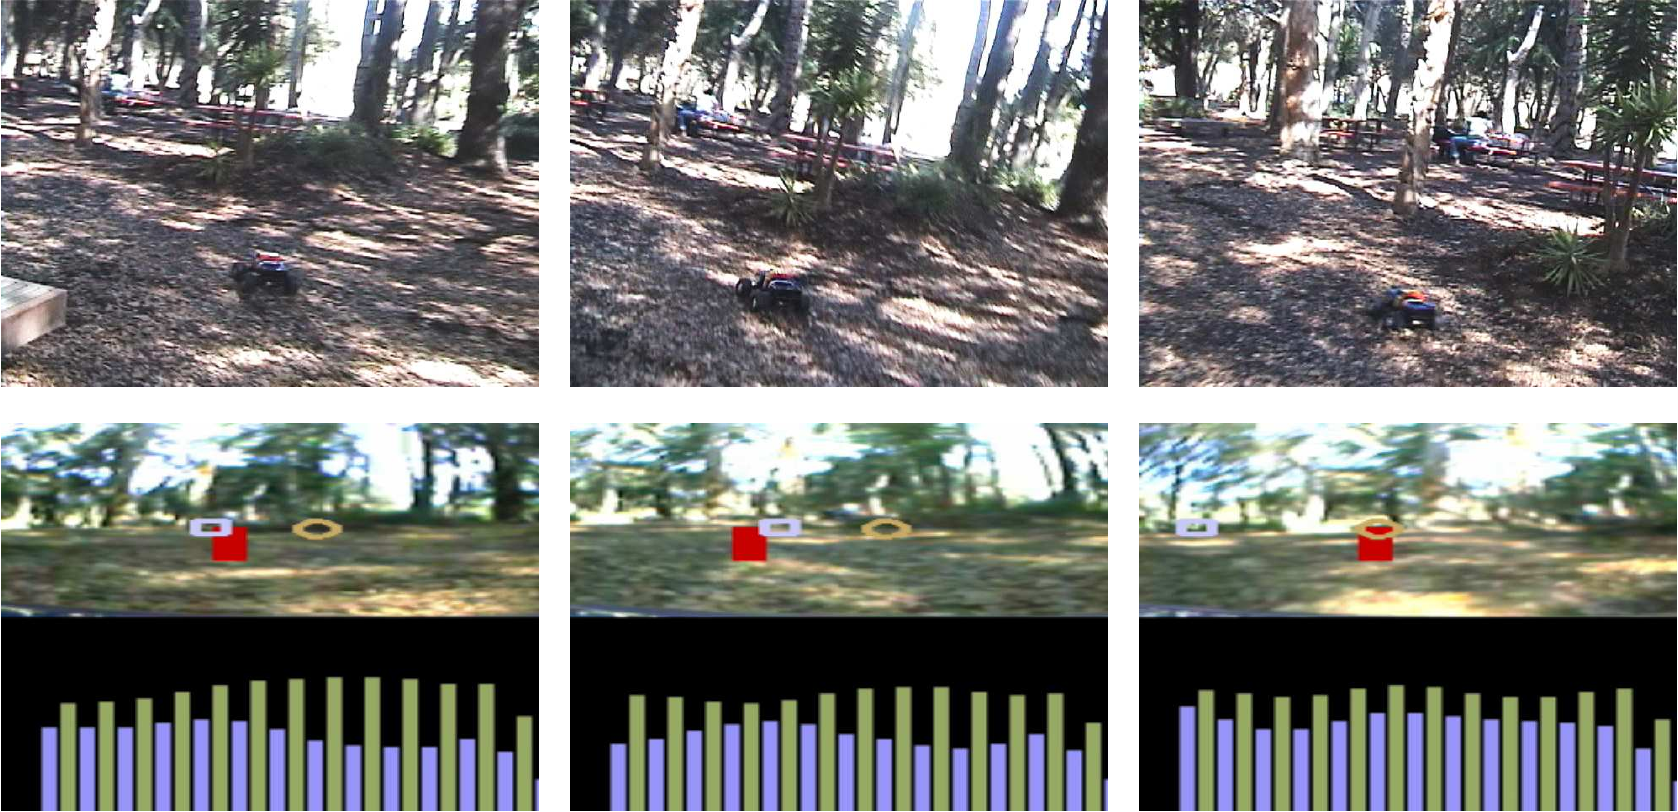
\includegraphics[width=\textwidth]{RC_car}
\caption{Une séquence d'images montrant l'évitement d'un obstacle}
\end{figure}

\section{Apprentissage de la profondeur d'une seule image}

Saxena et al.\cite{saxena2005learning} ont travaillé sur l'estimation de la
profondeur d'une seule image par l'utilisation d'un apprentissage supervisé.
Les images et les cartes de profondeur sont collectées à partir des scènes de
l'extérieur fortement destructurées contenant plusieurs objets (arbres, bâtiments, etc).

Contrairement à Michels and all, les images sont divisées en de petites
pièces servant à calculer les vecteurs de caractéristiques sur différentes
échelles en utilisant des masques de convolution.

\begin{figure}[H]
\begin{center}
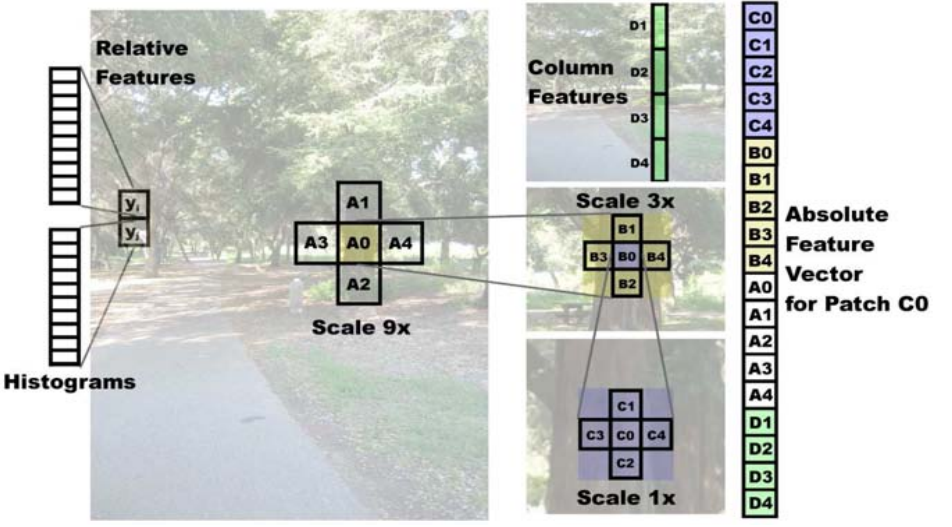
\includegraphics[width=0.75\textwidth]{FeaturesVectorScales}
\caption{Le vecteur de caractéristiques à  différentes échelles}
\end{center}
\end{figure}

De plus, il ont choisi la technique du \keyword{champ aléatoire de Markov} comme
méthode d'apprentissage car elle est un modèle probabiliste permettant de
prendre en considération les corrélations existantes entre pièces adjacentes.
Ils ont commencé par la variante gaussienne du modèle, puis ils ont
basculé vers la laplacienne vu qu'elle est la plus adaptée à ce problème.
La figure suivante présente quelques résultats de leurs expériences, la première
colonne représente l'image, la deuxième c'est la carte des profondeurs réelles, et
les deux dernières sont les cartes de profondeurs générées par le modèle gaussien
et le modèle laplacien respectivement.

\begin{figure}[H]
\begin{center}
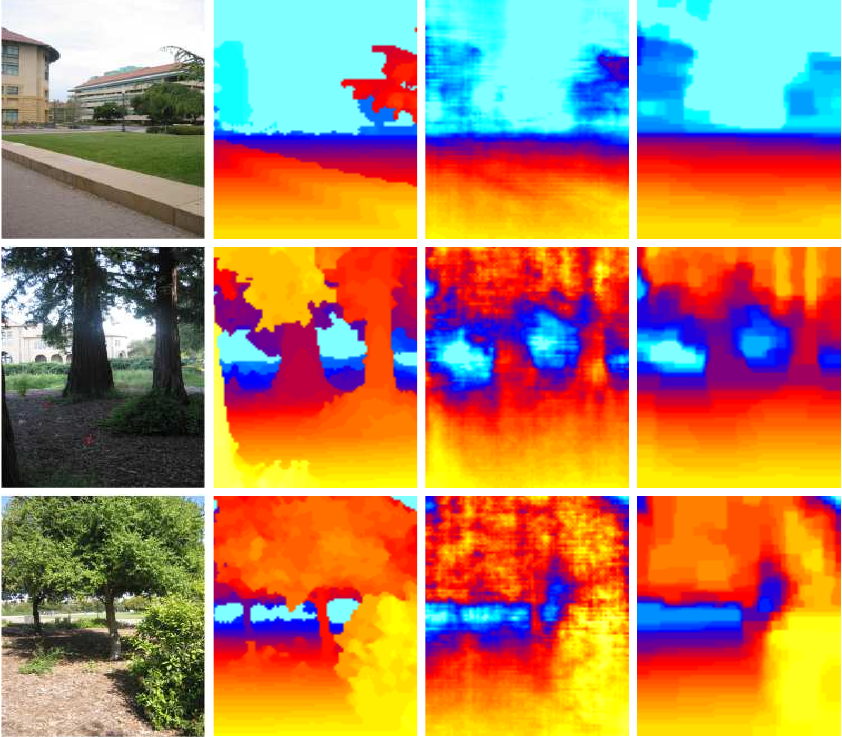
\includegraphics[width=0.75\textwidth]{DepthLearningResults}
\caption{Quelques résultats de l'apprentissage de profondeur}
\end{center}
\end{figure}

Dans un autre travail, Saxena et al.\cite{saxena2009make3d} ont aussi utilisé les
\keyword{champs aléatoires de Markov}
pour estimer la structure 3D détaillée d'une scène. De même, leur travail -qui
s'appelle \keyword{Make3D}- repose sur l'utilisation d'apprentissage supervisé et
sur la vision monoculaire. Ils ont décomposé chaque image en un ensemble de
triangles appelés \keyword{superpixels} où chacun représente une surface planaire.
Les informations de la profondeur sont utilisées de la même manière que dans les
travaux précédents, mais en ajoutant des contraintes géométriques permettant de
traiter plus de cas. Ils ont réussi à transformer plusieurs images 2D en
images 3D. Ils ont aussi étendu leur projet pour utiliser d'autres informations
quand c'est possible, comme les relations entre les objets dans une seule image, ou
la différence de vues pour une photo. La figure suivante montre des photos
utilisées dans leurs tests avec les résultats obtenus.

\begin{figure}[H]
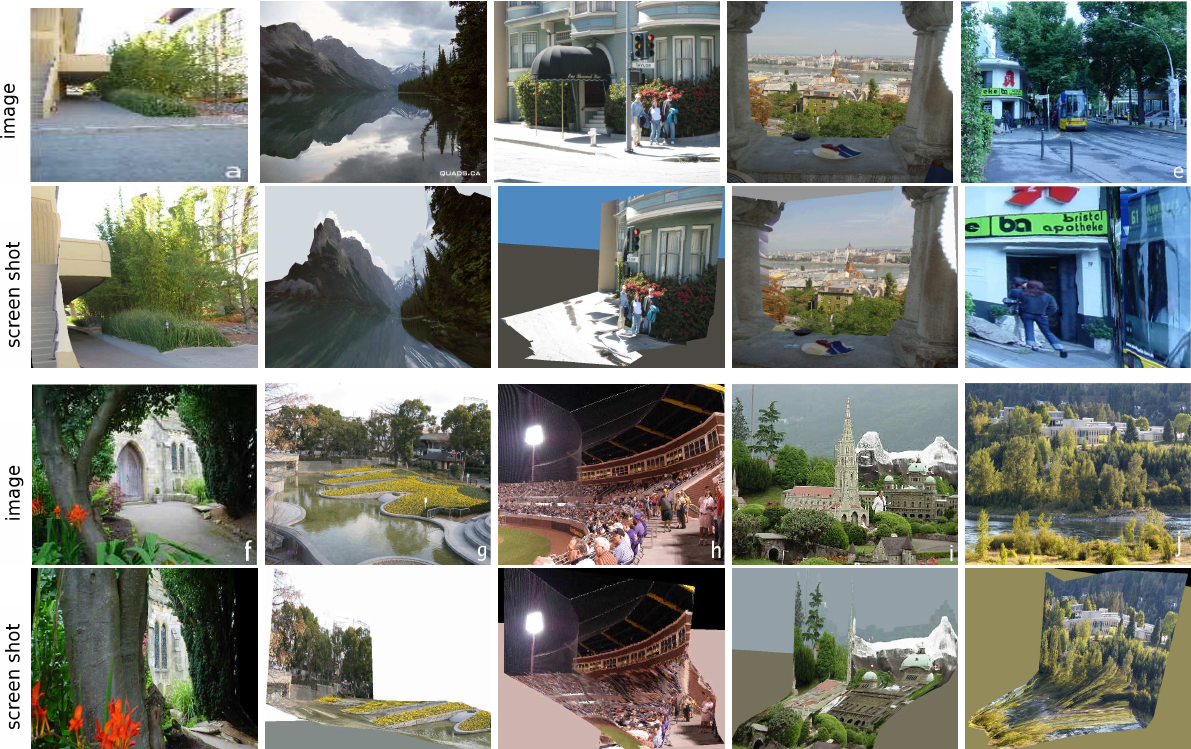
\includegraphics[width=\textwidth]{make3D_tests}
\caption{Quelques images transformées en 3D avec Make3D}
\end{figure}

\section{Les réseaux de neurones convolutionels pour l'estimation de la profondeur}

Un des travaux récents qui ont utilisé les \keyword{réseaux de neurones convolutionels}
pour l'estimation de profondeur est celui de Eigen et al.\cite{eigen2014depth}.

L'approche consiste à développer un réseau de neurones convolutionel consitué de
deux niveaux. Le premier prédit la profondeur à un niveau global, tandis que le
deuxième applique des raffinements successifs afin de générer une carte des
profondeurs plus précise. Les deux niveaux acceptent l'image originale comme
entrée. De plus, la sortie du premier niveau est fournie comme entrée pour
le deuxième.

Ils ont entraîné ce modèle par les ensembles de données de \keyword{NYU v2} qui
contient des scènes d'intérieur de maison, et de \keyword{KITTI} qui est un ensemble
de scènes d'extérieur. Les résultats obtenus après l'apprentissage étaient
généralement meilleurs que ceux de \keyword{Make3D}, et cela est dû à la
structure multi-échelles du réseau qui permet de combiner la vue globale avec les
vues locales sur l'image.

\begin{figure}[H]
\begin{center}
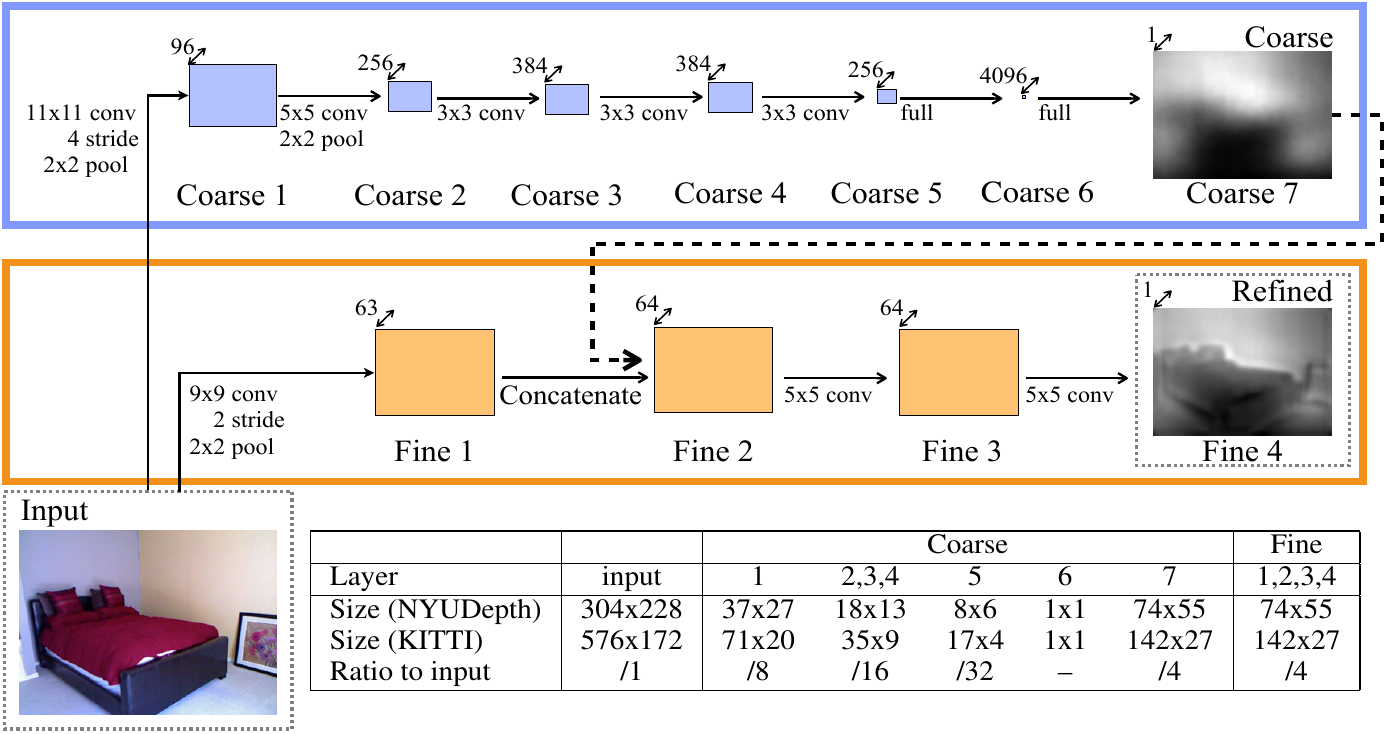
\includegraphics[width=0.6\textwidth]{Double_CNN_Architecture}
\caption{L'architecture du réseau à deux niveaux}
\end{center}
\end{figure}

\vspace{-1em}

Dans un travail ultérieur, Eigen et Fergus\cite{eigen2015predicting} ont étendu
le modèle précédent par l'ajout de deux autres fonctionnalitées : l'estimation
de la normale de chaque surface et l'étiquetage sémantique. Ils ont gardé le
principe de réseaux multi-échelles qui ne nécessite aucun prétraitement de bas
niveau.

La nouvelle architecture de ce modèle est formée de trois sous réseaux
convolutionels dont le résultat de chacun et l'image originale sont alimentés
au suivant, les sous-réseaux étant plus profonds que ceux du travail précédent.
Le premier permet de prédire des caractéristiques globales sur toute l'image.
Le second produit des prédictions d'un niveau moyen de détails en intégrant les
informations du premier. Le dernier affine ces prédictions pour générer une
sortie à un haut niveau de détails en utilisant toutes les informations précédentes.

\vspace{1em}

\begin{figure}[H]
\begin{center}
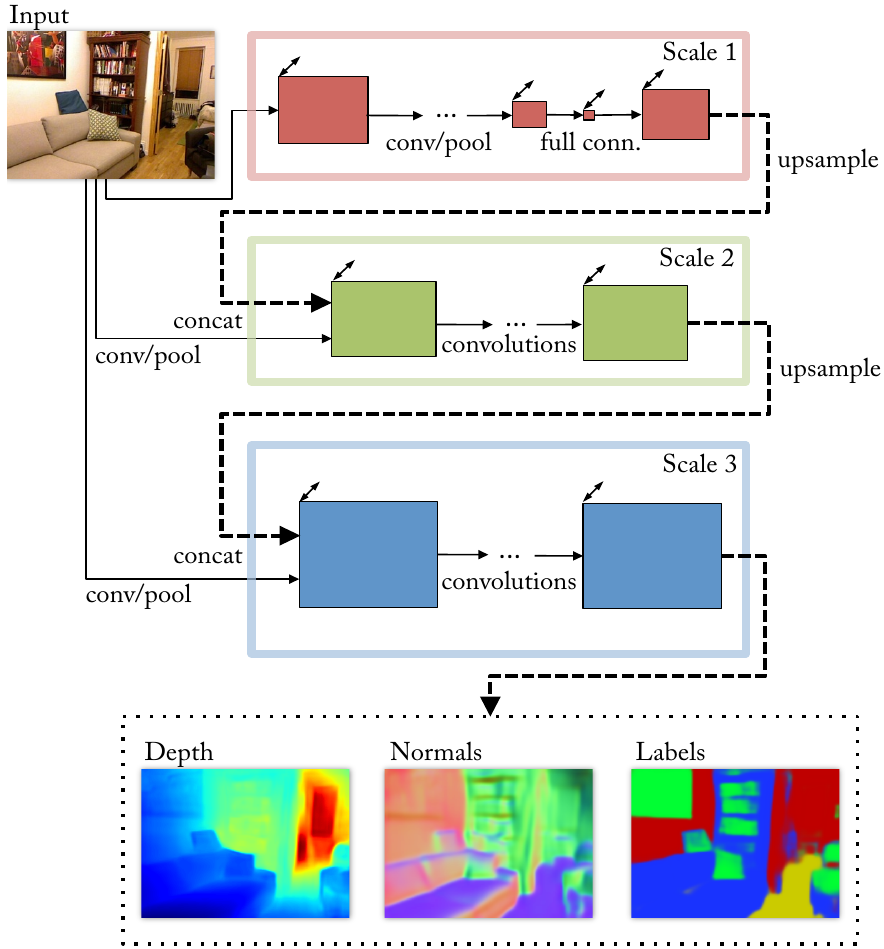
\includegraphics[width=0.5\textwidth]{CNN_Multi_Architecture}
\caption{L'architecture du réseau à trois niveaux}
\end{center}
\end{figure}

\section{Les champs de neurones convolutionels}

Liu et al.\cite{liu2015deep} ont créé un modèle hybride qui bénifice de la combinaison
des \keyword{réseaux de neurones convolutionels} avec les \keyword{champs aléatoires
conditionnels} (CRF) pour l'estimation de la profondeur. Le modèle est composé de deux
parties : une partie qui calcule les similarités par paires entre les
\keyword{superpixels} voisins qui sont transmis à une couche entièrement connectée,
et l'autre partie qui est un réseau convolutionel constitué de cinq couches
convolutionelles suivies par quatre autres entièrement connectées. Le résultat
de chacune de ces deux parties est fourni à la couche finale qui calcule la
probabilité de chaque profondeur en utilisant la formule de CRF.

\begin{figure}[H]
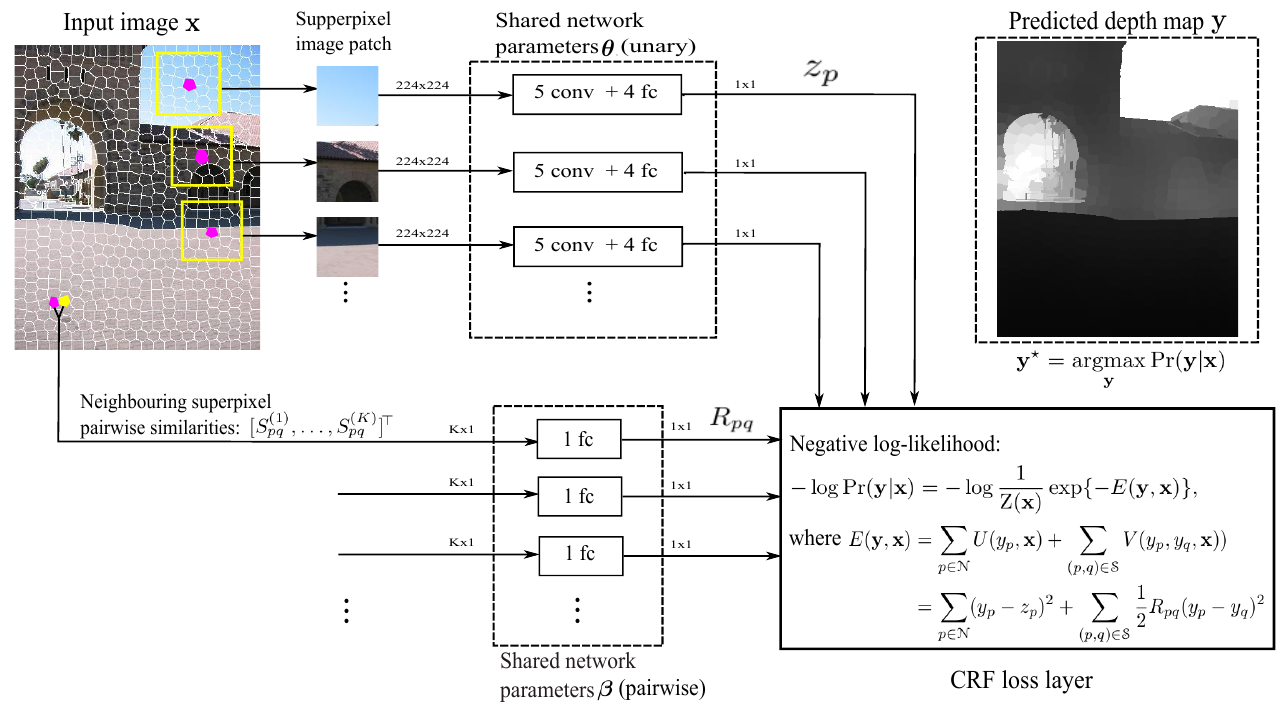
\includegraphics[width=\textwidth]{CRF_CNN_Architecture}
\caption{L'architecture globale du champ de neurones convolutionel}
\end{figure}

L'apprentissage a été effectué après avoir initialisé les couches par les poids
d'\keyword{ImageNet} en utilisant l'ensemble de données de \keyword{Make3D} et de
\keyword{NYU v2}. Ce travail a dépassé toutes les méthodes existantes pour
ces deux ensembles de données.

\section{Conclusion}

Dans ce chapitre nous avons présenté quelques travaux antérieurs concernant
l'estimation de distances ou de profondeurs à partir d'une seule image.
Toutes ces méthodes utilisent les ensembles de données contenant des cartes de
profondeurs générées à partir des scanners laser (comme SICK et Microsoft Kinect)
car ils sont très précis pour calculer la distance d'un point.
Cependant, ils ont quelques inconvénients, comme leur poids qui ne peut pas être négligeable
et leur sensibilité à la lumière du soleil qui peut fausser les calculs, ce que
les rend peu pratiques pour l'utilisation dans les appareils qui peuvent être
exposés aux rayons solaires. De plus, il sont relativement coûteux.

A notre connaissance, tous les projets d'estimation de distances précédents
n'ont utilisé que les scanners lasers. De ce fait, nous avons essayé d'utiliser
une autre option : les capteurs ultrasoniques. Bien que leur précision soit
relativement plus faible que celle des scanners laser et que leur taux d'erreur
puisse être élevé dans les scènes contenant des objets avec des surfaces
irrégulières, ils ont des avantages comme leur légèreté et leur insensibilité
à la lumière, et de plus, leur coût est très faible.

Dans le chapitre suivant nous présenterons les parties matérielles et logicielles
formant notre projet qui est un robot constiué de plusieurs composants et
programmé pour pouvoir se déplacer en prenant des photos de l'environnement
avec les distances respectives.

% \chapter{La machine de l'acquisition des données}

\section{Introduction}

L'objectif de ce travail, en premier lieu, est d'avoir un ensemble de données
composé d'images d'environnement avec un certain nombre de distances qui
représentent  les écarts respectifs entre la position de l'appareil permettant
de prendre chaque image et les obstacles qui sont y visibles.

Afin d'atteindre ce but nous avons vu la nécessité de fabriquer une machine mobile
permettant l'acquisition de ces données d'une manière automatique. La machine que
nous avons réalisé nous facilite la tâche et accélère énormément le rythme du travail.
De ce fait, nous pouvons obtenir une quantité importante de données dans un temps
réduit.

Cette machine possède une capacité limitée de navigation automatique, mais
elle peut être télécommandée par un ordinateur à travers une connexion sans fil
entre le programme qui s'exécute sur l'ordinateur et les programmes qui ordonnent
la machine. L'ensemble de ces programmes avec le matériel forment un système
qui a pour rôle de collecter les données nécessaires pour l'étape de
l'apprentissage automatique.

Le système est composé d'une partie matérielle et d'une autre logicielle. Chaque
partie sera présentée à part en montrant les détails de son fonctionnement.

\section{La partie matérielle}

La construction physique du robot est composée d'une carcasse et de plusieurs
parties électroniques, chaque partie offrant au moins une fonctionnalité
élémentaire. Les parties principales sont :

\begin{itemize}
  \item quatre moteurs de courant continu,
  \item un pilote de moteurs \keyword{L298N},
  \item des capteurs ultrasoniques \keyword{HC-S04},
  \item un moteur servo \keyword{TowerPro SG90},
  \item un capteur de température (et d'humidité) \keyword{DHT22},
  \item un microcontrôleur \keyword{Arduino Mega 2560},
  \item un appareil équipé du système d'exploitation \keyword{Android},
  disposant d'une camera RGB et d'un port USB qui permet la connexion en série
  (dans notre cas, nous avons utilisé un téléphone \keyword{Samsung Galaxy Note 2})
  \item une source d'alimentation électrique qui peut fournir une intensité de
  courant suffisante pour faire fonctionner les moteurs et les capteurs (nous
  avons utilisé une banque d'alimentation électrique combinée avec des piles).
\end{itemize}

\subsection{Le pilotage des moteurs}

Un moteur de courant continu tourne dans une seule direction à la fois. Cette
direction est déterminée par le sens du courant traversant la bobine interne
du moteur. La direction de la rotation peut être inversée seulement en inversant
le sens du courant électrique. De plus, l'intensité de ce courant détermine la
vitesse à laquelle ce moteur tourne.

\begin{figure}[h]
\begin{center}
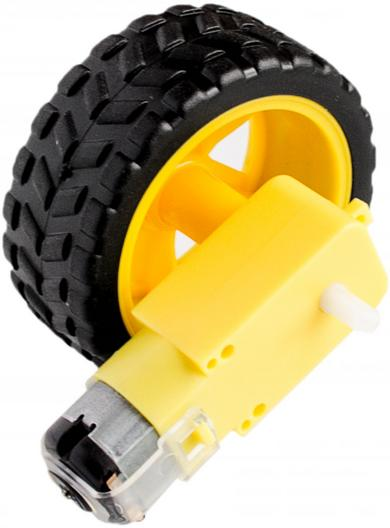
\includegraphics[width=0.2\textwidth]{DC_motor_wheel}
\caption{Le moteur de courant continu utilisé avec la roue}
\end{center}
\end{figure}

Pour pouvoir manipuler ces paramètres (le sens et la vitesse de la rotation), il
faut utiliser un pilote de moteurs comme \keyword{L298N}. Ce module peut contrôler
deux moteurs indépendamment, chacun dans un sens et à une vitesse donnée. Cependant, il est
aussi capable de gérer plus de deux moteurs, à condition qu'ils soient distribués
en deux groupes de telle manière que tous les moteurs du même groupe fonctionnent
par les mêmes paramètres.

Dans ce travail, nous avons eu recours à quatres moteurs
(pour supporter le poids du véhicule), chaque paire étant considérée comme un
seul groupe et située dans un côté du véhicule (droite ou gauche).
Les moteurs d'un côté tournent toujours dans le même sens avec la même vitesse.
La variance du sens entre les deux côtés détermine le type de mouvement : si
tous les moteurs tournent dans le même sens, alors le robot avance ou recule
selon le sens de la rotation, et si les moteurs des différents côtés tournent dans
des sens différents, alors le robot tourne autour de lui-même.

\begin{figure}[h]
\begin{center}
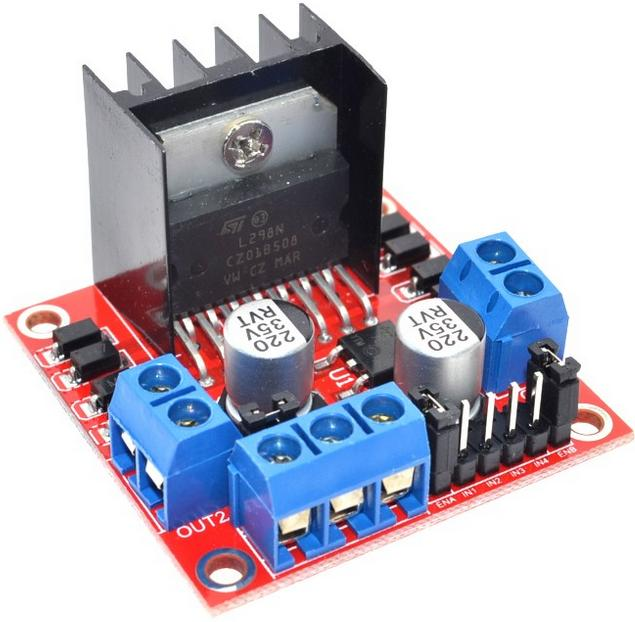
\includegraphics[width=0.3\textwidth]{L298N}
\caption{Le contrôleur de moteurs L298N}
\end{center}
\end{figure}

\subsection{La mesure de distances}

Les capteurs ultrasoniques sont des composants qui permettent l'envoi et la
réception du signal ultrasonique. En effet, ils sont utilisés pour le calcul
de la distance d'un objet. Pour ce faire, le capteur est commandé afin d'émettre
un signal dans une direction spécifiée. Si le signal ne frappe aucun objet avant de
s'affaiblir, il sera perdu et la distance ne pourra pas être calculée; sinon il
retournera au capteur à qui il notifiera le circuit commandant par la réception.
Par la suite, le circuit peut calculer la différence entre les instants d'émission
et de réception et utilise cette durée pour estimer la distance en connaissant
la vitesse du son dans l'air. La distance $d$ ($m/s$) est estimée par la formule suivante :

\begin{equation}
  d = t \times c \div 2,
\end{equation}

où $t$ est le temps écoulé en secondes entre l'envoi et la réception du signal,
et $c$ est la vitesse du son dans l'air sec et est approximée par la formule :

\begin{equation}
  c = 0.6 \times T + 331.4,
\end{equation}

avec $T$ la température de l'environnement en Celsius ($ ^\circ C$).

Afin de déterminer la température de l'air, nous avons utilisé le capteur
\keyword{DHT22} qui permet un relèvement de la température chaque $2$
secondes avec une haute précision (la marge d'erreur est seulement $\pm 0.5 ^\circ C$).

Ce capteur fonctionne en mode numérique. Il est activé seulement quand il reçoit
un signal approprié. Il renvoie le résultat à travers le même port au circuit
instantanément après avoir pris les mesures nécessaires.

\begin{figure}[h]
\begin{center}
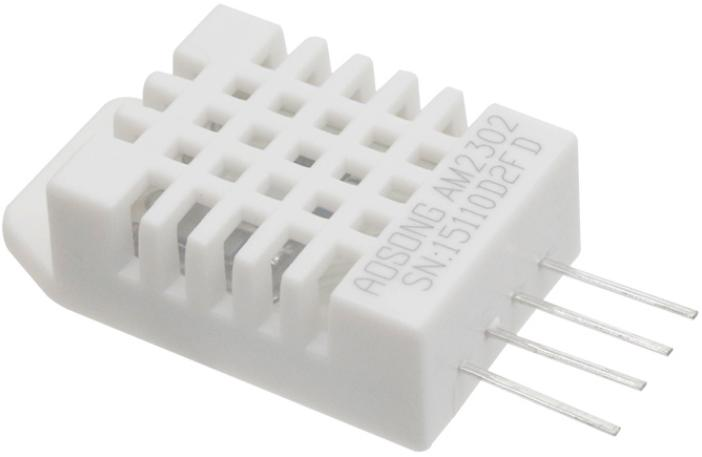
\includegraphics[width=0.25\textwidth]{DHT22}
\caption{Le capteur de la température DHT22}
\end{center}
\end{figure}

En outre, les capteurs d'ultrason opèrent sur une seule direction à la fois. Si
nous voulons avoir un ensemble de distances pour les différents obstacles éventuels
visibles dans le champ de vision du robot, nous avons besoin de plusieurs capteurs.

Mieux encore, on peut n'en utiliser qu'un seul et le faire tourner sous plusieurs
angles afin de couvrir la zone de vision.
Pour cela, il faut monter le capteur ultrasonique sur le bras d'un \keyword{servomoteur}.
Ces moteurs ont la capacité de déplacer leur bras par des angles exacts compris
généralement entre $0^\circ$ et $180^\circ$. Le circuit de contrôle envoie l'angle
d'inclinaison du bras au servomoteur qui effectue cette opération mécanique rapidement.
Nous avons utilisé le servomoteur \keyword{TowerPro SG90} pour cette tâche.

\begin{figure}[h]
\begin{center}
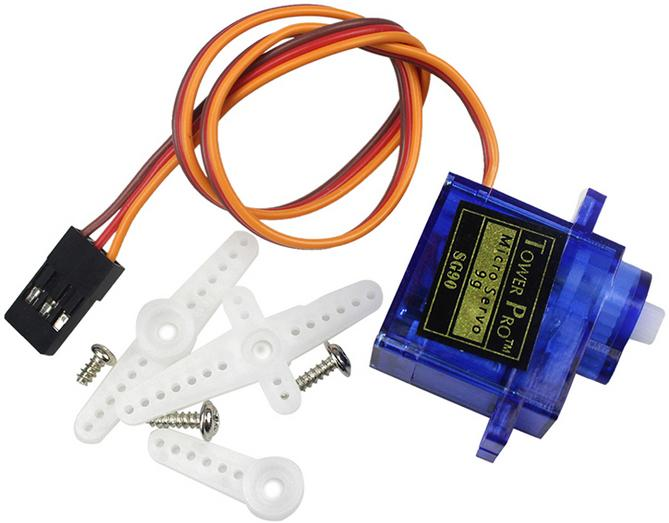
\includegraphics[width=0.3\textwidth]{SG90}
\caption{Le servomoteur TowerPro SG90}
\end{center}
\end{figure}

\subsection{Le contrôle des composants}

Afin de contrôler tous les modules précédents, il nous faut un microcontrôleur.
Dans ce travail, nous avons utilisé une version compatible avec le
microcontrôleur \keyword{Arduino Mega 2560}.

Nous avons connecté les ports de données de ce microcontrôleur aux autres
composants (le pilote de moteurs, le capteur ultrasonique, le capteur de la
température et le servomoteur) en utilisant des câbles compatibles après avoir
placé tous ces modules dans leurs positions respectives. Par la suite, il sera
chargé par un programme permettant de gérer continuellement les autres modules
par l'envoi de commandes ou par la réception d'informations.

\begin{figure}[h]
\begin{center}
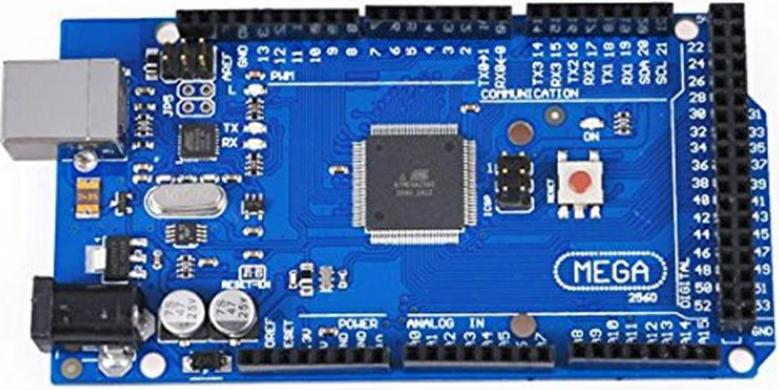
\includegraphics[width=0.3\textwidth]{ArduinoMega2560}
\caption{Une version compatible avec le microcontrôleur Arduino Mega 2560}
\end{center}
\end{figure}

Il y a deux types de ports : les \keyword{ports numériques} à lecture et
écriture, et les \keyword{ports analogiques} à lecture seule. Certains ports
numériques supportent \keyword{la modulation de largeur d'impulsion} et donc peuvent
émettre un signal composé d'une succession d'états discrets de <<tout ou rien>>
pendant une unité de temps dont la fréquence est choisie par le programme.

Étant donné que les performances du microcontrôleur sont très limitées, nous
devons le connecter à un appareil plus puissant en termes de vitesse
de calcul et de capacité en mémoire, et disposant d'autres options comme la
mise en réseau. Afin de satisfaire ces besoins, nous avons intégré le téléphone
intelligent \keyword{Samsung Galaxy Note 2} comme partie du robot en le connectant
par un cable USB avec le microcontrôleur. Cela permet d'établir une connexion en série entre
ces deux appareils, après avoir développé une application s'exécutant
sur le téléphone et permettant l'échange d'informations avec le microcontrôleur
en même temps qu'avec l'ordinateur hôte.

\begin{figure}[H]
\begin{center}
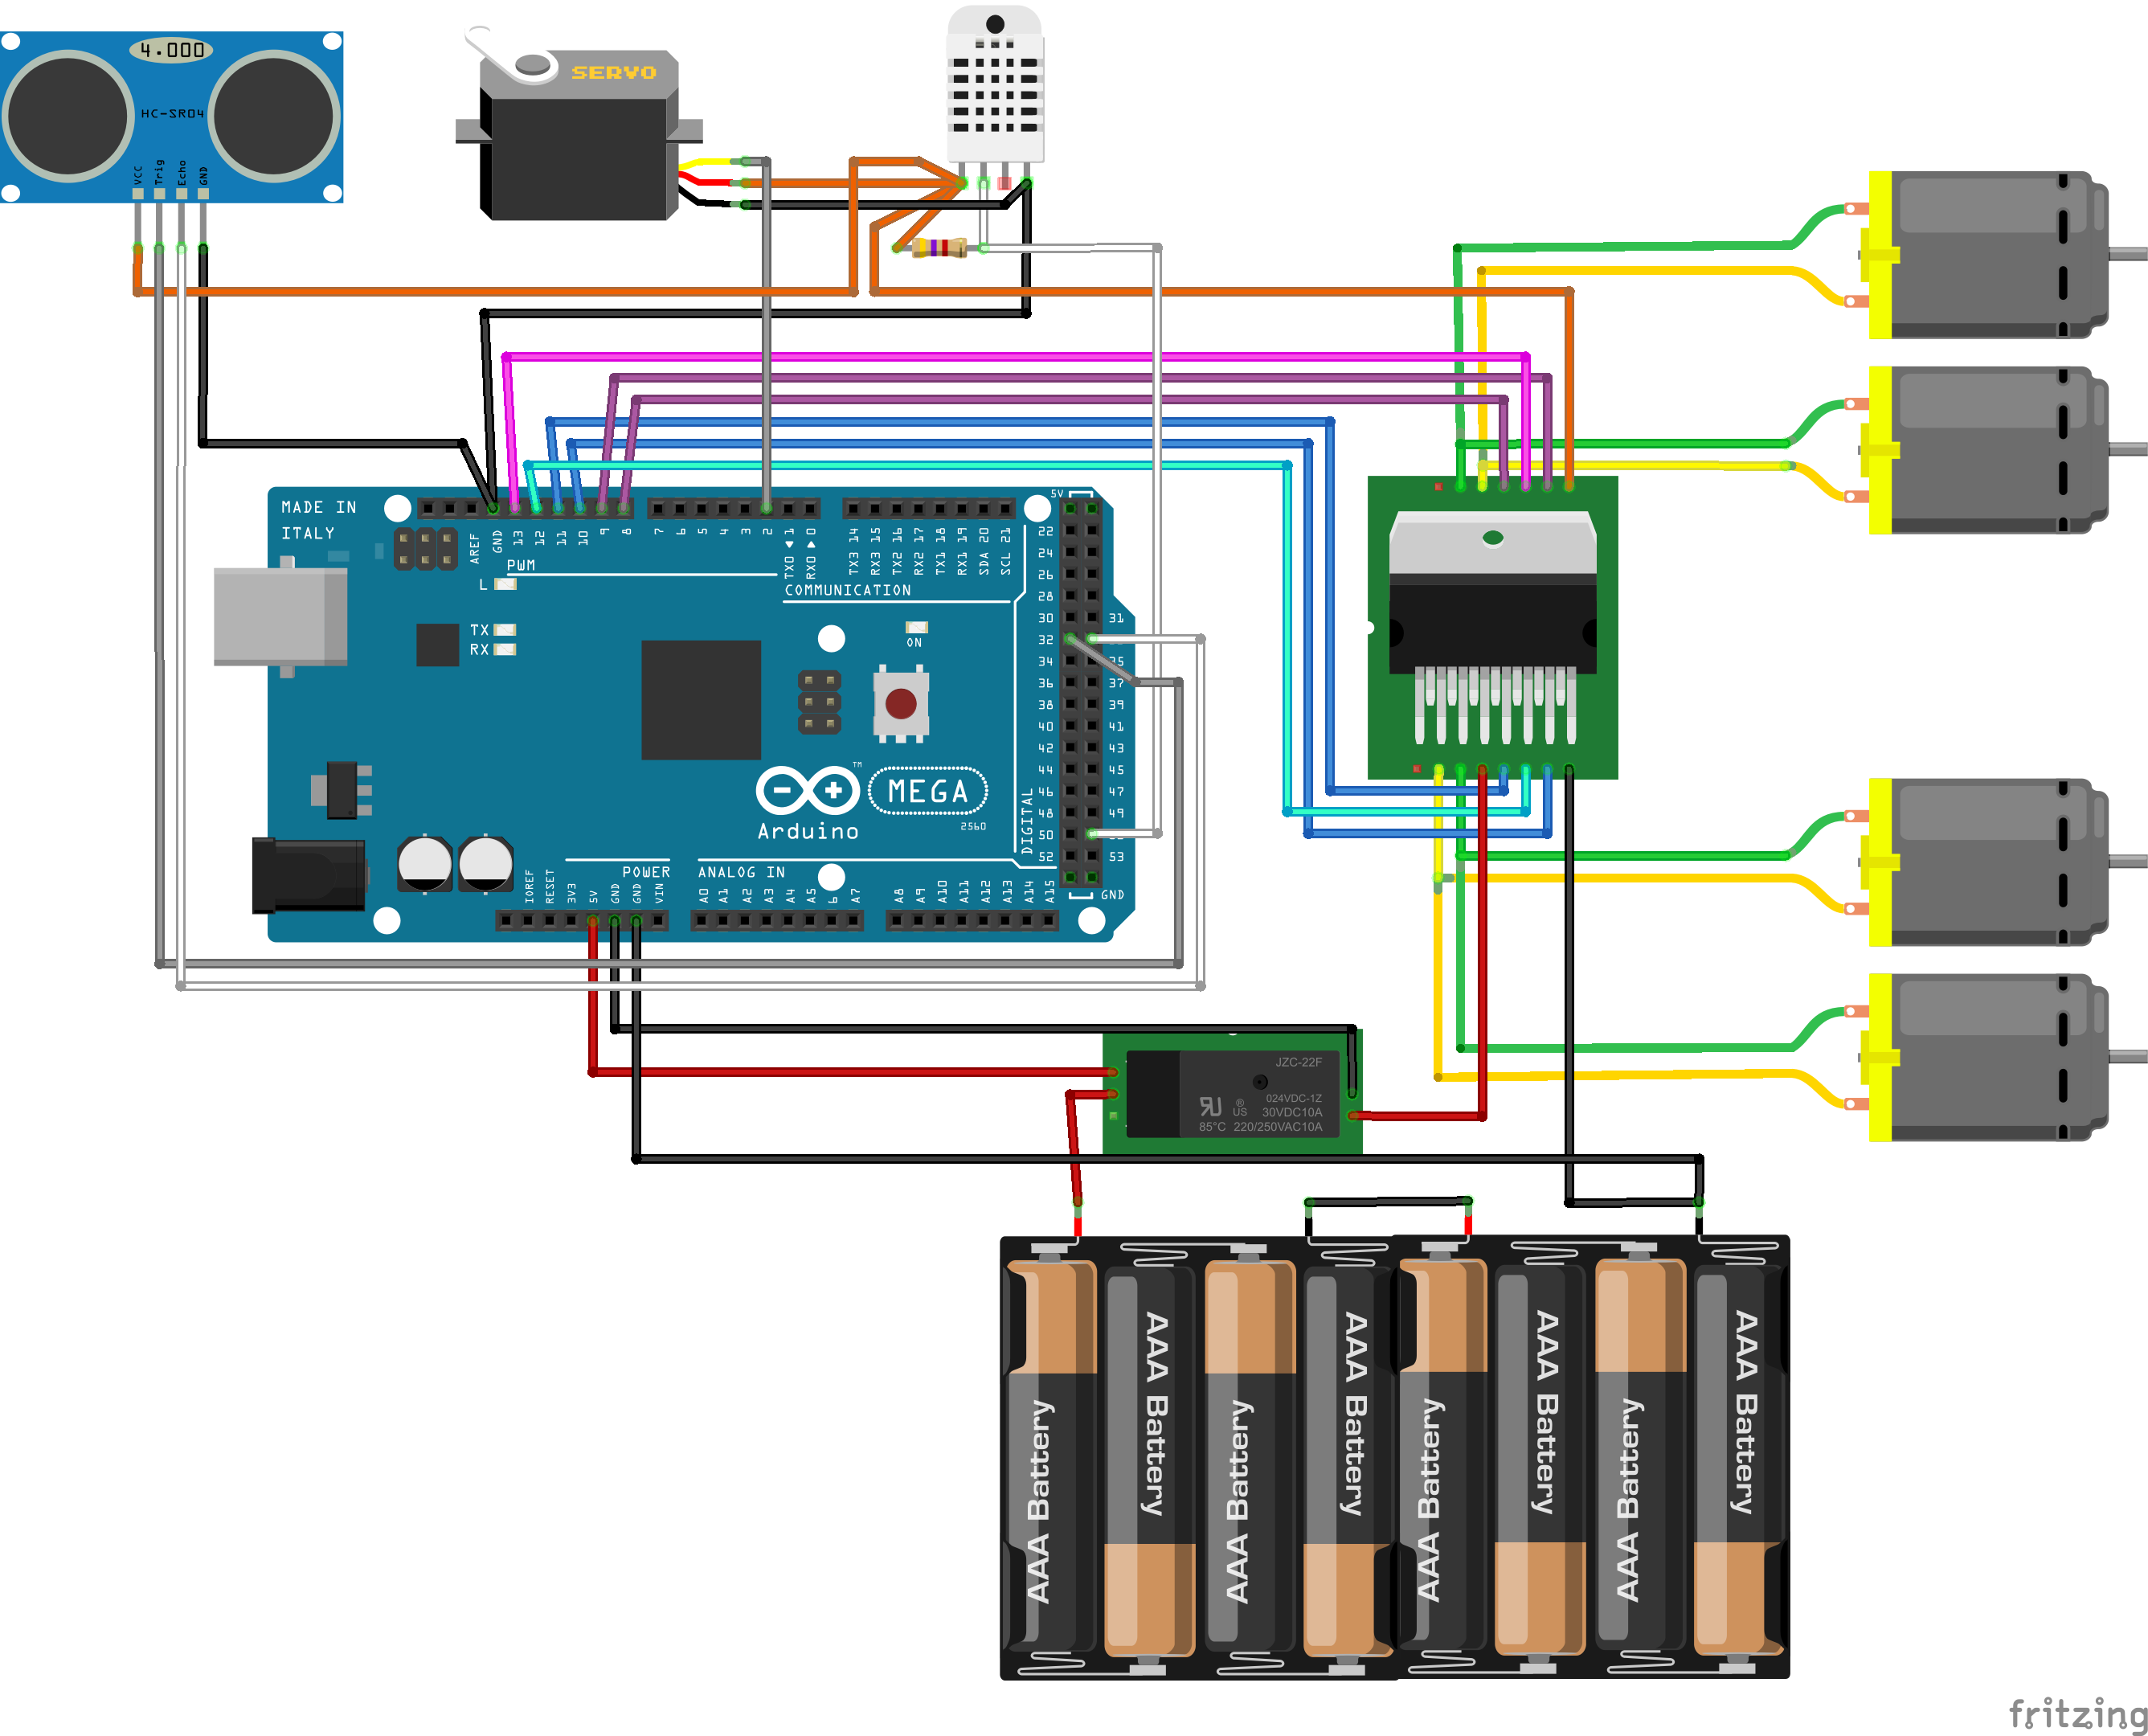
\includegraphics[width=0.7\textwidth]{DistancesRobotCircuit}
\caption{Le schéma des connexions entre les modules du robot}
\end{center}
\end{figure}

Jusque là, nous avons présenté les composants matériels nécessaires pour la
construction du robot et la manière dont ils sont utilisés en indiquant la
fonctionalité de chacun d'eux. Dans la partie suivante nous présenterons les
logiciels développés pour chaque plateforme et nous expliquerons leur fonctionnement
ainsi que leur intercommunication qui permettent la gestion du robot.

\begin{figure}[h]
\begin{center}
  \begin{subfigure}{0.49\textwidth}
    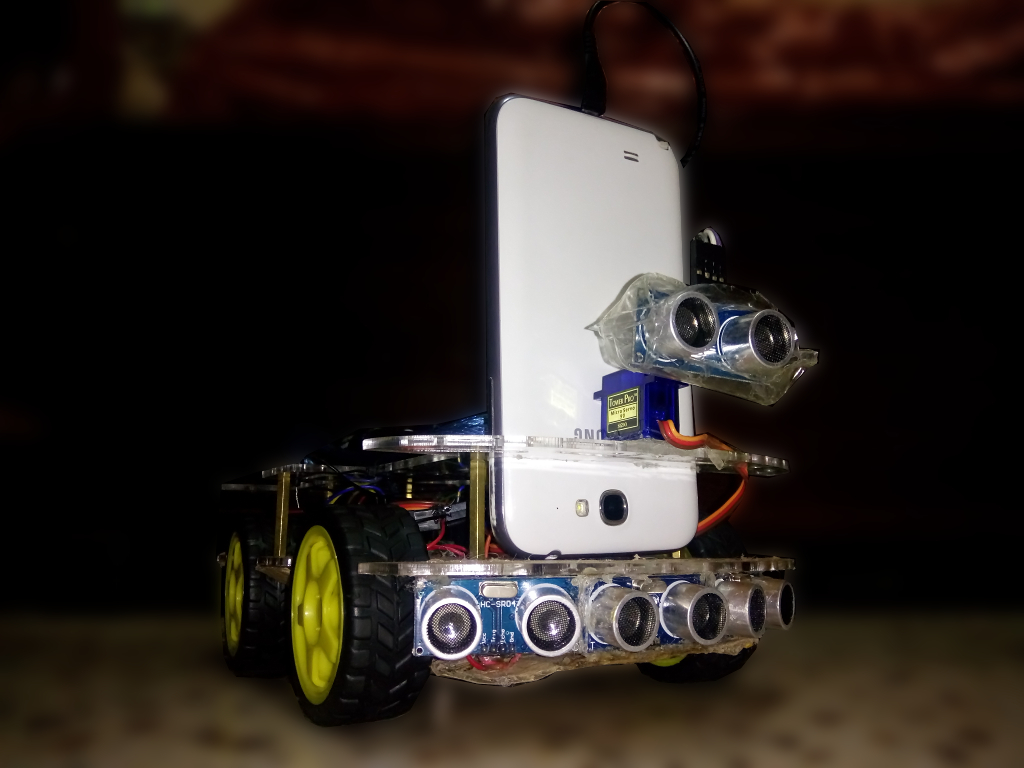
\includegraphics[width=\textwidth]{Distances_robot_front}
    \caption{Vue de face}
  \end{subfigure}
  \hfill
  \begin{subfigure}{0.49\textwidth}
    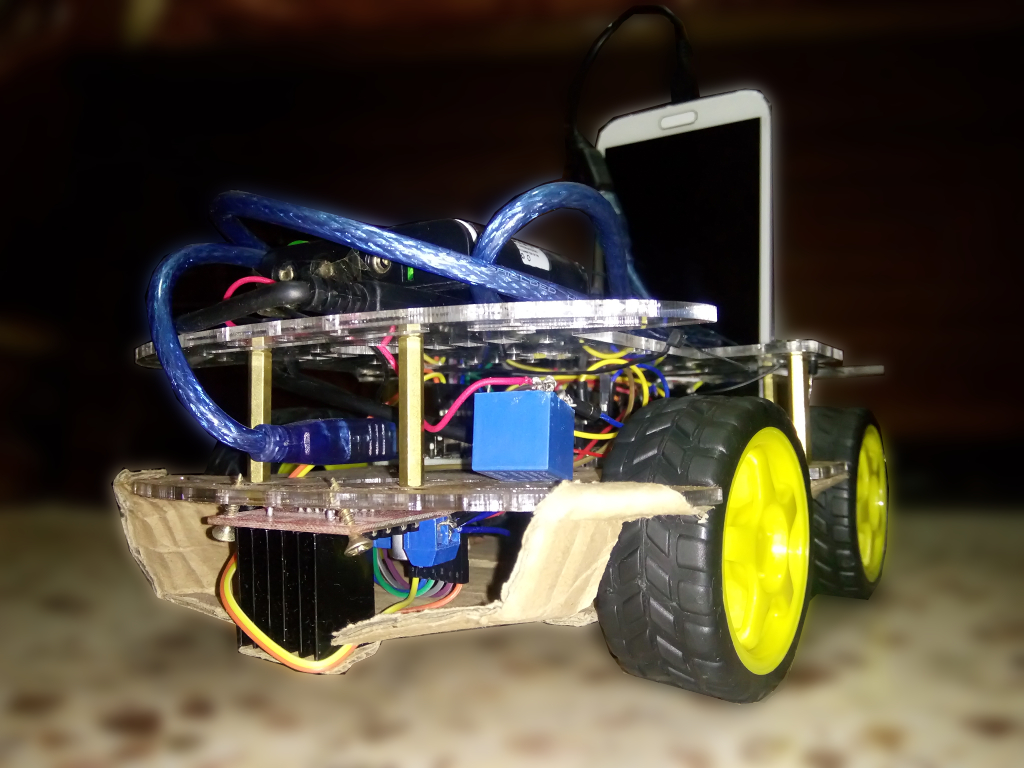
\includegraphics[width=\textwidth]{Distances_robot_back}
    \caption{Vue arrière}
  \end{subfigure}
  \caption{Des photos du robot}
\end{center}
\end{figure}

\section{La partie logicielle}

L'ensemble des composants du robot est géré directement par deux logiciels, l'un
s'exécute sur le microcontrôleur, et l'autre sur le téléphone. Ce dernier
envoie des commandes à l'autre qui contrôle directement le matériel.

\subsection{Le programme du microcontrôleur}

C'est un programme répétitif, testant à chaque fois s'il y a
une commande reçue par le téléphone à travers la connexion en série. Si c'est le cas,
il teste le nom de la commande pour savoir quelle action il faut exécuter.
Une fois que l'action et ses paramètres éventuels sont déterminés, un signal
approprié est envoyé au module correspondant qui exécute cette action et renvoie
éventuellement une réponse. Cette réponse qui est déterminée par l'environnement
est capturée par le microcontrôleur et traitée à ce niveau avant de la propager
au téléphone.

Ce programme reconnaît plusieurs commandes, chacune étant représentée par un
caractère. Si la commande nécessite un paramètre (par exemple le changement de la
puissance des moteurs), le caractère de la commande est suivi par une chaîne de
caractères contenant la valeur du paramètre. Cette valeur est toujours un nombre
entier.

Si l'action performée en reconnaissant une commande retourne un résultat (par
exemple la température), il est envoyé au téléphone comme une chaîne de
caractères. Le téléphone traîte le résultat comme nous détaillerons dans la prochaine partie.

L'algorithme suivant présente le fonctionnement général du programme du
microcontrôleur. Il est constitué d'une boucle infinie (c'est-à-dire qu'elle
s'exécute tant que l'appareil est allumé) qui attend la réception d'une commande
et puis teste son type afin d'effectuer l'action nécessaire.

\smallskip

\begin{algorithm}[h]
\caption{Le programme du microcontrôleur}
\BlankLine
\While{le microcontrôleur est allumé}{
  \If{il y a une commande reçue}{
    \Switch{la commande}{
      \Case{distances}{
        Mesurer les distances et les envoyer\;
      }
      \Case{mouvement}{
        Tourner/Arrêter les moteurs\;
      }
      \Case{température}{
        Prendre la température et l'envoyer\;
      }
      \Case{puissance}{
        Ajuster la puissance des moteur\;
      }
    }
  }
}
\end{algorithm}

La commande de distance ordonne au microcontrôleur d'envoyer des signaux
successifs au servomoteur pour le faire tourner d'un angle à chaque fois ($10$ degrés
dans notre cas). La durée entre l'envoi d'un signal et le suivant est fixée dans
le programme afin de réserver la durée nécessaire pour l'opération mécanique (qui
est la rotation du bras du servomoteur). En même temps, la distance vers le
premier obstacle est mesurée à chaque angle par l'envoi d'un autre signal au capteur
de distances monté sur le servomoteur. La mesure de distance n'est pas toujours
possible : si l'objet est très loin (plus de $4.5m$) ou si sa surface est inclinée
ou irrégulière, alors l'ultrason envoyé sera perdu et la distance ne peut pas être
déterminée. Dans ce cas, une valeur constante et grande sera mise à la place de la
distance réelle pour indiquer qu'elle est inconnue. L'ensemble de distances est
transféré par la suite au téléphone par le biais de la connexion en série.

Les commandes de mouvement sont les quatre commandes de direction (avancer, réculer
tourner à droite et tourner à gauche) et la commande d'arrêt. Lors de la
réception de la commande d'arrêt, le microcontrôleur ordonne au pilote des moteurs
de couper le courant passant dans tous les moteurs, ce qui cause leur arrêt. Dans
le cas de la commande d'avancement ou de recul, tous les moteurs sont alimentés
par un courant de même sens dont un sens provoque l'avancement et l'autre cause
le recul. Le même principe s'applique pour tourner le robot, sauf que le courant
passant par les moteurs d'un côté est l'inverse de celui passant par les moteurs
de l'autre côté.

La commande de relèvement de la température est exécutée pour
mettre à jour la valeur de celle ci dans la mémoire et l'afficher à l'utilisateur.
Cette valeur est indispensable pour le calcul de la vitesse du son dans l'air
dans l'environnement courant. Le relèvement est fait par l'envoi d'un signal spécial
au capteur qui renvoie la température courante au microcontrôleur.

Toutes les actions citées précédement ne sont exécutées que à la réception de
la commande correspondante à partir de l'application du téléphone que nous expliquerons
son fonctionnement dans ce qui suit.

\subsection{L'application du téléphone}

Elle a pour rôle de commander
le microcontrôleur et d'en recevoir des informations. Les informations
sont utilisées pour faire des calculs et prendre des décisions sous
forme d'actions. Certaines sont également envoyées au logiciel qui s'exécute sur
l'ordinateur. De plus, elle prend périodiquement des images en utilisant la camera
du téléphone.

L'application envoie une commande de température après chaque intervalle de temps
($2$ secondes) au micrôcontrolleur. Dès la réception de sa valeur, elle met à
jour son interface graphique et l'envoie à l'ordinateur.

De même, l'application envoie la commande de distances et prend une photo périodiquement
(chaque $0.3$ seconde). Les distances retournées et la photo prise sont sauvegardées
temporairement dans deux files, chaque file correspondant à un type d'objets.
\`A chaque fois, un élément de chaque file est défilé et selon le mode
de la capture et la fréquence de la sauvegarde (qui est fixée à $1$ instance de
données par seconde), ces éléments peuvent être enregistrées de façon permanente
dans la mémoire externe.

L'envoi des commandes de mouvement dépend directement du mode de la navigation.
Si le mode est automatique, l'envoi est exécutée après chaque intervalle de temps
(qui est égale aussi à $0.3$ seconde). Dans ce cas, l'application décide quelle
commande il faut envoyer en utilisant les distances précédents.
Si le mode est manuel, l'envoi est effectué seulement quand l'application reçoit
un ordre explicite de l'utilisateur.

La commande de changement de puissance est toujours exécutée seulement
à l'ordre de l'utilisateur. Elle contient la valeur de la puissance qui
est un nombre entier définit sur l'intervalle $[0-255]$. Cette valeur est initialisée
par défaut à $127$.

Cette application acte également comme un pont entre l'ordinateur et le microcontrôleur
en utilisant deux types de connexions : une connexion en série par câble entre
le téléphone et le microcontrôleur, et une autre sans fil par Bluetooth entre
le téléphone et l'ordinateur. Les connexions restent toujours ouvertes
mais les transferts n'ont lieu qu'à certains moments. Ces transferts peuvent
se faire dans les deux sens et sont soit périodiques soit apériodiques selon l'action.

Les actions périodiques sont :
\begin{itemize}
  \item le relèvement de la température de l'air dans l'environnement,
  \item le choix de la direction de la navigation,
  \item la sauvegarde des données sur le périphérique du stockage externe (la carte mémoire).
\end{itemize}

\bigskip

Les actions apériodiques sont :
\begin{itemize}
  \item l'envoi de commandes de mouvement issues de l'utilisateur,
  \item le changement de la puissance des moteurs,
  \item le lancement et l'arrêt de la capture et de la navigation.
\end{itemize}

\subsection{Le logiciel de l'ordinateur}

Il offre une interface qui permet à l'utilisateur
de contrôler le robot à distance et de garder un œil sur son état. Il affiche la
température de l'air où se situe le robot et le nombre de données capturées et
sauvegardées sur la mémoire permanente. Il permet aussi de signaler quelques
erreurs causées par le matériel comme le dysfonctionnement de la camera.

\begin{figure}[h]
\begin{center}
  \begin{subfigure}{0.4\textwidth}
    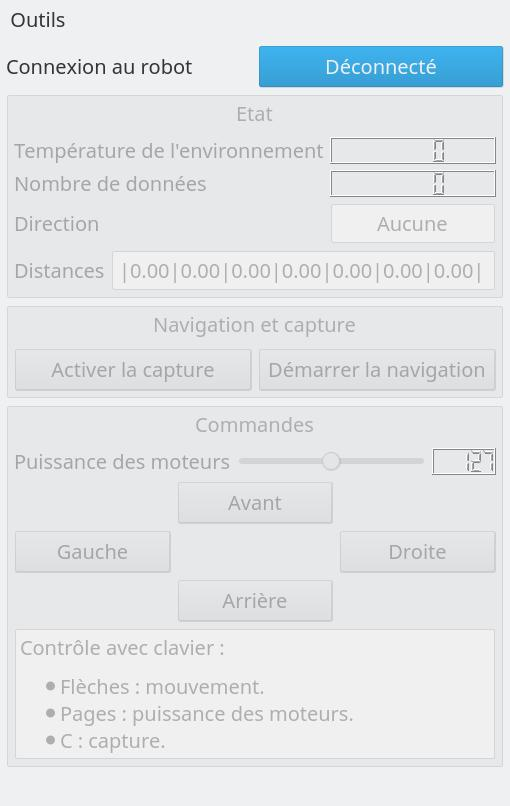
\includegraphics[width=\textwidth]{ComputerControler}
    \caption{\'Etat \textbf{déconnecté}}
  \end{subfigure}
  \hspace{2em}
  \begin{subfigure}{0.4\textwidth}
    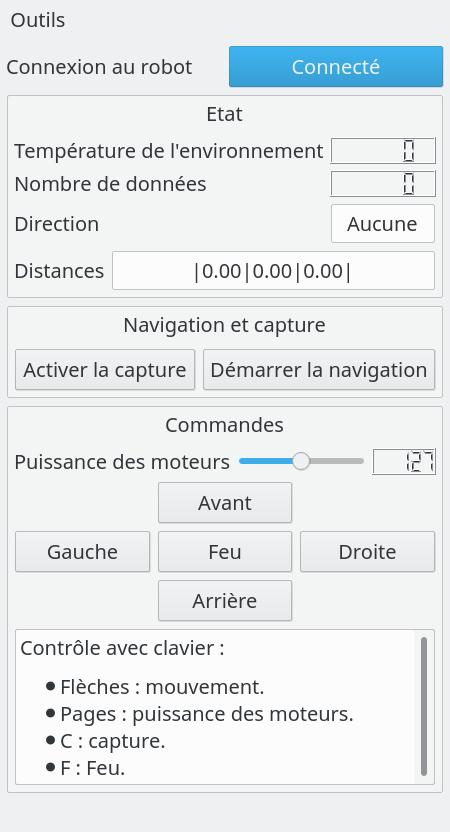
\includegraphics[width=\textwidth]{ComputerControler_connected}
    \caption{\'Etat \textbf{connecté} avec navigation}
  \end{subfigure}
  \caption{L'interface principale du logiciel d'ordinateur}
\end{center}
\end{figure}

Le logiciel permet de guider de façon directe le robot en envoyant des commandes
de direction (avant, arrière, droite et gauche) ou un signal de
navigation automatique. Il permet également de changer la puissance des moteurs
et d'activer ou de désactiver la sauvegarde de données capturées.
La sauvegarde peut être effectuée indépendamment
du mode de navigation, c'est-à-dire qu'elle peut être activée sans que la
navigation soit automatique et vice versa.

Les commandes de mouvement et de sauvegarde peuvent être activées par les
boutons existant sur l'interface ou par des touches de clavier. Les instructions
permettant de guider la machine par n'importe quelle méthode sont clairement visibles
sur l'interface.

Ce logiciel offre une autre interface qui a pour fonction de visualiser les
données collectées en affichant à la fois une photo capturée avec les distances
respectives en mètres.

\begin{figure}[H]
\begin{center}
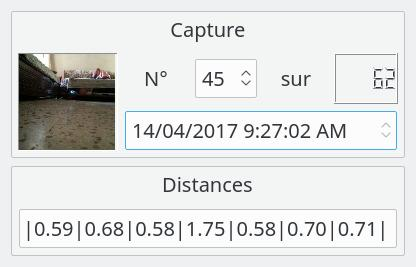
\includegraphics[width=0.4\textwidth]{CapturesViewer}
\caption{L'interface de la visualisation des données}
\end{center}
\end{figure}

\section{La collecte et le traitement des données}

Après avoir allumé le robot et lancé les programmes nécessaires, il peut commencer
à effectuer la tâche d'acquisition. Il se déplace et prend périodiquement une image
de taille $480 \times 640$, ensuite il coupe ses marges haute et basse par un
déplacement de $80$ pixels sur chaque marge, ce qui aboutit à une image carrée
de $480 \times 480$ pixels. La taille de l'image est par la suite réduite à
$96 \times 96$ pixels pour des raisons d'économisation de l'espace de stockage
et d'optimisation des calculs de l'apprentissage automatique qui sera effectué
ultérieurement. Chaque image est sauvegardée comme un fichier qui porte comme
nom un préfixe (\texttt{IMG\_}) suivi par un identificateur numérique généré
au moment de la capture (l'\keyword{époque}\footnote{Elle représente le nombre de
millisecondes passées depuis le premier janvier 1970 à minuit dans le temps
universel coordonné (UTC).}). En même temps, dans un autre fichier, les distances
correspondant à chaque image sont enregistrées avec l'identificateur de cette
dernière, chaque instance étant écrite sur une ligne. Le nombre de distances
est fixé à $3$ par image. Si la distance ne peut être mesurée, alors une valeur
constante ($9.99$) est insérée pour indiquer que la distance est manquante.

\section{Conclusion}

Dans chaque problème d'apprentissage automatique, un ensemble de données considérable
est nécessaire pour pouvoir effectuer cette tâche. Cette nécessité nous a mis devant
deux choix : utiliser un ensemble de données prêt où les données sont collectées
et traitées par d'autres personnes, ou bien construire notre propre ensemble en
utilisant nos propres outils que nous devons développer nous-mêmes.

Nous avons choisi la deuxième méthode. De ce fait, nous avons
fabriqué le robot dont nous avons décrit la construction matérielle et la
programmation au niveau logiciel. Il nous a permis de collecter les images
prises au niveau de sa vision et les distances des obstacles éventuels dans
chaque image.

Dans le chapitre suivant, nous allons exploiter ces données grâce à
un apprentissage automatique supervisé en utilisant la méthode de
réseaux de neurones convolutionels.

% \chapter{L'apprentissage supervisé avec les réseaux de neurones convolutionnels}

\section{Introduction}

Après la construction de notre base de données qui contient les images avec
les distances respectives, nous pouvons entamer la création du modèle qui
permettra l'estimation de distances à partir d'images en appliquant un
apprentissage supervisé sur les données. Nous proposons donc notre propre
architecture d'un réseau de neurones convolutionnel.

Nous commençons par la description de la structure de nos
données et les prétraitements appliqués sur ces données. Ensuite, nous présentons
les réseaux convolutionnels que nous avons conçus pour effectuer l'apprentissage
selon notre approche.
Par la suite, nous exposons notre méthode d'apprentissage et les paramètres
que nous avons choisis pour le réaliser.

\section{Les données et les prétraitements}

Nous avons pris des données à partir de plusieurs sources pour construire des
ensembles de données. Chaque ensemble contient un nombre considérable d'images et
de distances dont chaque image correspond à un nombre de distances ($3$ distances
pour chacune). Les images représentent les entrées du modèle et les distances
représentent les sorties.

\subsection{Les distances}

Pour simplifier l'apprentissage, nous avons besoin de réduire le nombre de
distances prises à une seule distance par image. Cette opération doit être faite
à l'aide d'une fonction mathématique. Nous avons choisi d'appliquer la
\emph{médiane} après avoir éliminé les distances inconnues.

Par exemple, si on suppose qu'une image correspond aux distances $1.24$, $1.21$, $1.25$, la
distance choisie est $1.24$ car $1.21 < 1.24 < 1.25$. Par contre, si nous avons
les valeurs $0.95$, $9.99$, $0.89$, la distance choisie est $(0.95+0.89)/2 = 0.92$
car $9.99$ est une valeur numérique dont on considère qu'elle signifie que la distance est inconnue.
Elle sera remplacée par la valeur spéciale $NaN$\footnote{\keyword{Not a Number:
constante qui indique que la donnée n'a pas une valeur numérique valide.}}.
Dans ce cas, la médiane est équivalente à la moyenne.
De même, si nous avons seulement une seule distance connue, par exemple :
$9.99$, $9.99$, $0.67$, le résultat est cette valeur. Dans certaines instances,
il se peut que toutes les valeurs soient invalides, dans ce cas, nous somme obligés
de considérer la distance comme inconnue. La distance trouvée après ce traitement
est transformée en un vecteur binaire de $4$ cases où pour chaque distance il
y a une case mise à $1$ et les autres à $0$. Ce traitement permet de passer d'
un problème de régression à un problème de classification en distribuant
les distances comme il est indiqué dans le tableau suivant.

\begin{table}[h]
  \centering
  \begin{tabular}{|l|c|c|c|c|}
    \hline
    Classe & Petite & Moyenne & Grande & Inconnue \\
    \hline
    Intervalle & $[0,1.5[$ & $[1.5,3[$ & $[3,4.5[$ & $[4.5,+\infty[$ \\
    \hline
  \end{tabular}
  \caption{La distribution des distances (en mètres) sur les classes}
\end{table}

Par exemple, une distance de $1.75m$ appartient aux distances moyennes
selon le tableau, donc elle sera représentée par un vecteur $x$ de $4$ cases
où la deuxième contient la valeur $1$ et les autres contiennent $0$. Formellement,
nous représentons cela par la notation mathématique suivante.

$$ x =
\begin{pmatrix}
  0\\
  1\\
  0\\
  0\\
\end{pmatrix}
$$

Les distances inconnues sont représentées par la valeur constante $9.99$ et donc
appartiennent évidemment à la dernière classe.

\subsection{Les images}

Les images stockées ont une taille de $96 \times 96$ pixels et contiennent $3$
canaux dont chacun contient les valeurs d'une couleur parmi le rouge, le vert et
le bleu. Elles sont transformées au moment du chargement en images de niveaux
de gris qui n’ont qu’un seul canal. En même temps, elles sont réduites par un
facteur de $\frac{1}{2}$, ce qui donne des images de taille $48 \times 48$.
Ces petits prétraitements ont été effectuées afin de réduire la taille de données
fournies pour l'apprentissage, ce qui permet de l'accélérer significativement.

\begin{figure}[h]
\begin{center}
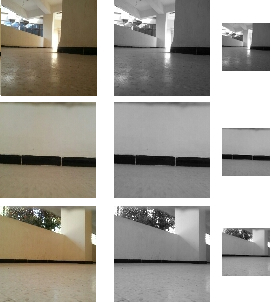
\includegraphics[width=0.4\textwidth]{Image-transformation}
\caption{Les prétraitements appliqués sur les images}
\end{center}
\end{figure}

\subsection{La transformation de données}

Afin d'alimenter nos modèles d'apprentissage, nous devons transformer l'ensemble
d'images et de distances en matrices multidimensionnelles portant les mêmes
informations. Les distances sont représentées par une matrice de deux dimensions :
la première pour les instances de distances dans un sous-ensemble, et l'autre pour
les classes d'une instance (dans notre cas il y a $4$). Par ailleurs, les images
sont représentées par une matrice de quatre dimensions dont la première correspond
aux instances, les deux suivantes à la hauteur et à la largeur
respectivement ($48$ pour les deux dans notre cas). La dernière représente le
nombre de canaux dans l'image ($1$ pour les images en niveaux de gris).

\section{Le modèle d'apprentissage}

Nous avons proposé deux architectures de réseaux de neurones convolutionnels composées
de plusieurs couches séquentielles de différents types. Ces architectures
séquentielles relativement profondes ont une structure inspirée de celle du
réseau \keyword{VGGNet} \cite{simonyan2014very}. La différence entre les deux
réside dans la profondeur et les hyperparamètres de chacune d'elles.

\begin{figure}[h]
\begin{center}
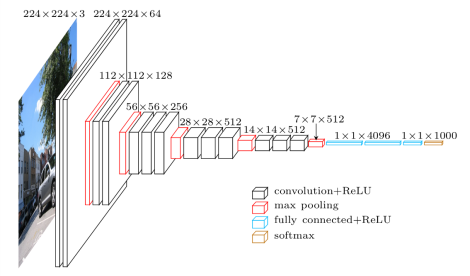
\includegraphics[width=0.5\textwidth]{imagenet_vgg16}
\caption{L'architecture de la variante du réseau VGGNet qui a 16 couches \cite{blier2016abrief}}
\end{center}
\end{figure}

\subsection{La description}

Les architectures sont composéss de grandes parties. Les premières sont
constituées de deux couches convolutionnelles suivies par une couche de regroupement,
tandis que la dernière est composée uniquement d'une couche dense. La
profondeur d'une couche convolutionnelle augmente d'une partie à une autre
bien que la taille spatiale de leur filtre diminue.

Le choix des couches convolutionnelles vient du fait qu'elles sont les plus
adaptées aux applications de la reconnaissance d'images car elles prennent en
considération la structure multidimensionnelle de l'image. De plus, vue que
chaque neurone de ces couches est connecté à un sous-ensemble de neurones de la
couche précédente, les paramètres dont le réseau doit apprendre sont moins nombreux et cela
est dû au \keyword{partage des paramètres}. Les sorties $z$ de chaque couche
convolutionnelle sont filtrées par la fonction d'activation ReLU (Rectified Linear Unit)
qui a la formule suivante.

$$
\mathrm{ReLU}(z) = \max(0,z) \cite{NIPS2012_4824}.
$$

Une couche de regroupement par le maximum est insérée après chaque ensemble de couches
convolutionnelles. Ce type permet de réduire la taille de l'image en appliquant
la fonction mathématique $\max$ sur les pixels adjacents dans chaque région. Cette
opération permet de réduire la variance intraclasse en diminuant les informations
inutiles. Pour chaque matrice de deux dimensions $A(N \times M)$, le regroupement
par le maximum $\mathrm{MaxPool}$ est défini par la formule suivante.

$$
\mathrm{MaxPool}(A) = \max(\{A_{n,m} | 1 \leq n \leq N, 1 \leq m \leq M\}) \cite{scherer2010evaluation}.
$$

Dans le dernier niveau du réseau, une couche dense est insérée afin de
rassembler tous les caractéristiques détectées à travers toute l'image, car cette
dernière contient des caractéristiques différents d'une région à une autre.
La couche de sortie est aussi une couche dense dont le nombre de perceptrons est
égale au nombre de classes (dans notre cas, c'est $4$). Les résultats $z$ sont
transmis vers la fonction $\mathrm{Softmax}$ afin de les normaliser pour
qu'ils représentent la probabilité dans l'intervalle $[0-1]$ de chaque classe.
Cette fonction est décrite par la formule suivante.

$$
\mathrm{Softmax}(z) = \frac{\mathrm{e}^{z_j}}{\sum^K_{k=1}\mathrm{e}^{z_k}}~\forall{j=\overline{1,K}} \cite{bridle1990probabilistic}.
$$

La raison pour laquelle l'architecture séquentielle est choisie est que les
couches peu profondes détectent
les caractéristiques de bas niveau (par exemple les lignes et les contours). Elles
ne sont pas nombreuses généralement, contrairement aux couches profondes qui détectent
les caractéristiques de haut niveau (comme les formes et les objets).
Cela est possible car la zone de couverture d'un neurone
augmente en parallèle avec sa profondeur.\cite{michael2015neural,Goodfellow-et-al-2016}

\subsection{La représentation textuelle}

L'architecture du réseau est sauvegardée comme un fichier texte sous le format
JSON (JavaScript Object Notation) \cite{introducing2012ecma}.
L'utilisation de ce type de fichier
permet de la créer, la copier et la modifier sans rien changer dans le
programme responsable de la construction du réseau. Elle est représentée comme un objet
ayant plusieurs attributs et leur valeur enregistrées dans un ordre précis.
Les attributs représentent les noms de couches et les valeurs contiennent
leur description. Chaque valeur est un objet contenant lui-même d'autres attributs
et d'autres valeurs dépendant du type de la couche décrite.

Les couches convolutionnelles ont quatre attributs :

\begin{itemize}
  \item \texttt{field\_size} : une valeur numérique entière strictement positive
  représentant la dimension horizontale et verticale du filtre de la convolution,
  \item \texttt{stride\_size} : une valeur numérique entière strictement positive
  représentant le pas de déplacement du filtre,
  \item \texttt{padding} : une des deux valeurs : \texttt{SAME} qui signifie
  l'utilisation de rembourrage par zéros, et \texttt{VALID} qui signifie le cas
  contraire,
  \item \texttt{depth} : une valeur numérique entière strictement positive représentant
  la profondeur de la couche, autrement dit, le nombre de matrices de paramètres
  partagées.
\end{itemize}

Les couches de regroupement par le maximum ont seulement les attributs \texttt{field\_size},
\texttt{stride\_size} et \texttt{padding} qui ont les mêmes sens. Les couches denses
n'ont que l'attribut \texttt{depth} qui dénote le nombre de perceptrons.

\subsection{La première architecture}

La première partie du réseau est constituée de deux couches convolutionnelles
ayant une profondeur égale à $16$ et dont la taille du filtre de chacune est
$5 \times 5$ déplacé par une unité à la fois, horizontalement et verticalement,
en ajoutant un rembourrage par zéros sur les quatre bords. Cela permet de garder
les dimensions originales de l'image entrante.
Elles sont suivies par une couche de regroupement par le maximum ayant un filtre
de taille $2 \times 2$ et un déplacement de $2$, ce qui réduit les dimensions de
l'entrée par un facteur de $\frac{1}{2}$. La deuxième partie est
identique à la première sauf que la profondeur de chaque couche convolutionnelle
est de $32$ et la taille du filtre de la convolution devient $3 \times 3$. Dans la
troisième partie, la couche dense contient $64$ perceptrons et elle est reliée
à toutes les sorties de la couche précédente. La couche de sortie est un
vecteur de taille $4$ où chaque perceptron représente une classe.

La figure suivante présente cette architecture. Les rectangles verts représentent
les couches convolutionnelles, les bleus représentent les couches de regroupement,
et les rouges représentent les couches denses.

\begin{figure}[h]
  \centering
  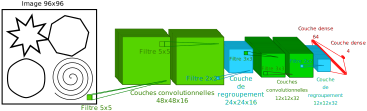
\includegraphics[width=\textwidth]{CNN1}
  \caption{Une représentation graphique de la première architecture}
\end{figure}

Le contenu du fichier qui décrit cette architecture est le suivant.
\lstinputlisting[caption=La représentation textuelle de la première architecture]
{../Code/PC/CNN-C5x16C5x16P2x2C3x32C3x32P2x2F64O4.json}

\subsection{La deuxième architecture}

Elle ressemble à la première mais elle est composée de quatre
parties principales. La première contient deux couches convolutionnelles ayant
un filtre de taille $7 \times 7$ et deux profondeurs de $8$ et $12$.
La deuxième contient des couches similaires dont le filtre a une taille de $5 \times 5$
et ses profondeurs sont de $16$ et de $24$. Les deux couches de la troisième parties ont
un filtre de taille $3 \times 3$ et des profondeurs de $32$ et $48$.
De même, une couche de regroupement est insérée après les deux couches
convolutionnelles dans les deux premières parties. Identiquement à l'architecture
précédente, celle-ci contient une couche dense de $64$ perceptrons dans la
dernière partie.

\begin{figure}[h]
  \centering
  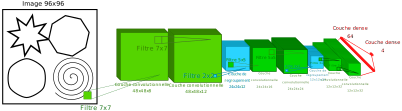
\includegraphics[width=\textwidth]{CNN2}
  \caption{Une représentation graphique de la deuxième architecture}
\end{figure}

\lstinputlisting[caption=La représentation textuelle de la deuxième architecture]
{../Code/PC/CNN-C7x8C7x12P2x2C5x16C5x24P2x2C3x32C3x48F64O4.json}

\section{L'apprentissage automatique du modèle}

Afin de rendre notre modèle opérationnel, nous devons changer ses paramètres en
appliquant un apprentissage supervisé par les données. En effet, nous devons
d'abord définir les modèles d'évaluation du réseau qui sont manipulés pour pouvoir
effectuer l’entraînement.

\subsection{La fonction de coût}

Les réseaux de neurones sont utilisés pour approximer des fonctions non linéaires.
Mais cette approximation n'est pratiquement jamais parfaite, il existe toujours
une quantité d'erreur entre les valeurs générées par le réseau et les valeurs réelles.
De ce fait, il faut définir une fonction permettant de calculer cette erreur et utiliser
une approche mathématique pour la minimiser.

Étant donné la transformation de ce problème vers une tâche de classification,
la formule d'erreur interclasses la plus adéquate est \keyword{l'entropie croisée}
qui est décrite par la formule :

$$
H(p, y) = -\sum_i y_i \cdot \log(p_i),
$$

avec $p$ le vecteur des valeurs calculées par le réseau et $y$ le vecteur des valeurs réelles.

Comme les valeurs de $y$ sont binaires, seulement la probabilité de l'élément de
la bonne classe qui sera prise en considération dans le calcul, et tous les autres
probabilités seront éliminées, et la somme de produits de logarithmes devient
juste un simple logarithme.
Par exemple, si nous avons comme données :

$$
y =
\begin{pmatrix}
  0\\
  1\\
  0\\
  0\\
\end{pmatrix}
~
\mathrm{et}
~
p =
\begin{pmatrix}
  0.6\\
  0.9\\
  0.3\\
  0.2\\
\end{pmatrix}
$$

la valeur de l'entropie croisée est calculée comme suit :

$$
H(p, y) = -(0 \times \log(0.6) + 1 \times \log(0.9) + 0 \times \log(0.3) + 0 \times \log(0.2))
$$
$$
H(p, y) = -\log(0.9) \approx 0.1054.
$$

\subsection{L'optimiseur}

L’apprentissage est effectué en minimisant la valeur d'erreur par une des fonctions
d'optimisation connus sous le nom d'\keyword{optimiseurs} qui sont basés sur la décente
du gradient. Cette dernière consiste à changer les poids du modèle dans les sens inverses
aux signes des dérivées partielles par un facteur nommé le \keyword{taux d'apprentissage}.
Il faut choisir et changer sa valeur avec précaution car une mauvaise valeur
risque d'empêcher l'optimiseur de converger vers l'optimum ou de gaspiller beaucoup
d'itérations pour ce faire.\cite{DBLP:journals/corr/Ruder16}

Dans ce travail, nous avons choisi l'optimiseur \keyword{Adadelta} \cite{DBLP:journals/corr/abs-1212-5701}
car il rend le choix du taux d'apprentissage sans aucune importance grâce à sa
formule de mise à jour de paramètres qu'elle les change indépendamment
selon la fréquence de modification de chacune à travers le temps.\cite{DBLP:journals/corr/Ruder16}

\subsection{L'exactitude}

Afin de pouvoir évaluer les performances d'un réseau de neurones, il faut définir
une formule d'exactitude permettant de calculer le nombre de résultats jugés
corrects par rapport au nombre total. La formule que nous avons utilisée est
la moyenne de comparaisons d'indices dont la valeur est maximale sur les
vecteurs de prédictions $P_i$ et les vecteurs d'étiquettes $Y_i$. Nous pouvons représenter
cela par la formule suivante.

$$
Acc = \frac{\sum_{i=1}^N(\mathrm{argmax}(P_i) = \mathrm{argmax}(Y_i))}{N},
$$

où $N$ est le nombre de vecteurs de prédictions dans l'ensemble et
$\mathrm{argmax}$ est la fonction qui donne l'indice de l'élément qui a la plus grande
valeur dans le vecteur numéro $i$.

\`A titre d'exemple, si nous avons les vecteurs de prédictions et les vecteurs
d'étiquettes suivants (représentés sous forme de matrices où les vecteurs sont transposés
et empilés sur la première dimension) :

$$
Y =
\begin{pmatrix}
  0 & \mathbf{1} & 0 & 0\\
  \mathbf{1} & 0 & 0 & 0\\
  0 & 0 & \mathbf{1} & 0\\
\end{pmatrix}
~
\mathrm{et}
~
P =
\begin{pmatrix}
  0.6 & \mathbf{0.9} & 0.3 & 0.2\\
  0.3 & 0.1 & \mathbf{0.7} & 0.5\\
  0.1 & 0.3 & \mathbf{0.5} & 0.1\\
\end{pmatrix},
$$

l'indice de l'élément ayant la valeur maximale sur chaque ligne dans les deux
matrices est le même pour les lignes $1$ et $3$, ce qui n'est pas vrai pour la
ligne $2$. L'exactitude dans ce cas est clairement égale à $\frac{2}{3} \approx 0.6667$
qui signifie que $66.67~\%$ de prédictions du réseau sont corrects.

\section{Conclusion}

Avant d'arriver à fixer la structure de nos données et choisir les différentes
architectures décrites dans ce chapitre, nous avons essayé plusieurs combinaisons
de variations de ces dernières que nous n'avons pas pu les mentionner.
Les tests que nous avons effectués ont montré les limitations de ces variations
en termes de complexité et vitesse d'exécution, et donc ils nous ont obligé de
transiter vers les modèles présentées ici.

Le prochain chapitre portera sur l'exécution de l'apprentissage automatique sur
ces modèles et ces structures en utilisant les ensembles de données que nous avons
collecté. Nous suivrons l'amélioration des performances du modèles et nous
enregistrerons les statistiques d'exécution obtenus en même temps.

% \chapter*{Conclusion générale}

Dans ce mémoire nous avons présenté notre projet qui est l'estimation de la distance
à partir des images en utilisant l'apprentissage automatique auto-supervisé.

Afin d'atteindre notre but, nous avons commencé par la construction d'une machine
électronique complexe constituée de plusieurs modules et de différents composants.
Elle est capable de se déplacer sur un terrain régulier, de mesurer
les distances des objets par rapport à son corps, et de prendre des images dans son
champ de vision.

Cette machine est commandée pour naviguer dans un espace fermé contenant éventuellement
des objets ayant des surfaces solides. En se déplaçant dans l'environnement, elle
prend périodiquement une photo et les distances des obstacles visibles. Les images
et les distances respectives sont sauvegardées dans un ensemble de données.

Par la suite, l'ensemble de données est fragmenté en deux : le grand sous-ensemble
est utilisé pour effectuer l'apprentissage du modèle, et l'autre est réservé
comme données de validation. En même temps, des réseaux de neurones convolutionnels
sont construits d'une telle structure permettant de réaliser l'objectif de ce projet.
Les modèles sont alimentés par les données d'apprentissage et sont testés par leurs
performances sont calculés en utilisant les données de validation jusqu'à atteindre
leurs limites d'amélioration.

Comme les résultats obtenus n'étaient pas très bonnes, nous avons pensé à des
idées qui peuvent perfectionner les modèles. Cependant, en raison de manque du temps et
de ressources humaines et matérielles, nous n'avons pas pu les réaliser et nous
les laissons donc comme perspectives.

Une idée est l'ajout plus de capteurs ultrasoniques et de meilleur qualité, ainsi
que la désactivation de capture au moment de déplacement du robot, et la réduction de
sa fréquence dans les autres moments. Cela permet de réduire le nombre de
distances fausses et les images floues causées par la vibration de la machine lors de la prise.

Une autre consiste à collecter beaucoup plus de données (des dizaines de milliers)
dans un seul environnement, puis les équilibrer avant le lancement de l'apprentissage,
car cette opération assure qu'il s'exécute correctement sans que les résultats soient
faussés par les poids des classes.

Une fois que les données deviennent nombreuses, il serait possible d'ajouter plus
que les quatre classes introduite dans ce travail afin d'obtenir un niveau supérieur
de précision. Il serait même possible d'aborder ce problème dans sa nature régressive.

Enfin, nous savons bien que ce travail est loin d'être parfait, mais il est le
premier -à notre connaissance- qui combine deux aspects : d'une part, la construction de la
machine permettant de collecter les données à l'aide \underline{des capteurs ultrasoniques}
et d'une camera ; et d'autre part, l'utilisation de ces données pour faire l'apprentissage
de nos propre modèles. Nous souhaitons que ce travail soit une initiative pour d'autres
recherches dans ce sujet.


\bibliographystyle{babplain}
\parskip=-1em
\bibliography{bibliographie}
\end{document}
